% Document template suitable for use as a LaTeX master-file 
% for thesis works in University of Turku Department of Computing
%
% Technical usage guide: https://tech.utugit.fi/soft/thesis/doc/doc/overview/
% 

\documentclass[language=english,version=final,mainfont=none,sharelatex=false]{utuftthesis}
\setcounter{secnumdepth}{2}
\setcounter{tocdepth}{2}
\usepackage{float}
\usepackage[caption=false]{subfig}
\usepackage{amsmath}
\usepackage{amssymb}
\usepackage{multirow}
\usepackage{booktabs}
\usepackage{graphicx}
\usepackage{array}

% Define the algorithm environment
%\makeatletter
\providecommand\textquotedblplain{%
  \bgroup\addfontfeatures{Mapping=}\char34\egroup}
\providecommand{\tabularnewline}{\\}
\floatstyle{ruled}
\newfloat{algorithm}{tbp}{loa}
\providecommand{\algorithmname}{Algoritmi}
\floatname{algorithm}{\protect\algorithmname}
%\makeatother

\addbibresource{Bibliografia.bib}

\begin{document}

\pubyear{2026}
\pubmonth{x}
\publab{TurkuNLP}
\publaben{TurkuNLP}
\pubtype{msc}
\title{Name of Thesis - To be decided}
\author{Miikael-Edvard Mändmets}

\maketitle
% \keywordsen{here, a, list, of, keywords}

\begin{abstracten}
Second abstract in english (in case the document main language is
not english)
\end{abstracten}



% mandatory
\tableofcontents

% if you want a list of figures
% \listoffigures

% if you want a list of tables
% \listoftables

% if you want a list of acronyms
% \listofacronyms

% change the name if the default doesn't sound right
% \renewcommand{\algorithmname}{\listingscaption}

% The thesis starts here.


\chapter{Introduction} \label{Introduction}

\section{Background and Motivation}

\label{Background and Motivation}

Large Language Models (LLMs) have fundamentally reshaped the landscape of artificial intelligence, demonstrating remarkable capabilities across natural language understanding, generation, and reasoning tasks. Building on this momentum, the field has increasingly moved toward Multimodal Large Language Models (MLLMs) that extend these capabilities beyond text to visual domains, enabling models to understand, generate, and manipulate images alongside language \cite{liu2023visualinstructiontuning, openai2024gpt4technicalreport}. Among the most rapidly advancing areas is AI-driven image generation and editing, which has seen dramatic improvements in both quality and controllability over recent years \cite{rombach2022highresolutionimagesynthesislatent, zhang2023addingconditionalcontroltexttoimage}.

A particularly consequential development has been the emergence of text-guided image editing, where users can modify images through natural language instructions rather than through manual, tool-based workflows. This paradigm shift lowers the barrier to image manipulation: tasks that previously required professional expertise in tools like Adobe Photoshop can now be performed by specifying the desired change in words \cite{adobe2023firefly}. However, not all image editing tasks are equal in difficulty. A useful distinction can be drawn between two categories of image editing that differ in how success is measured. We define qualitative editing as modifications to the semantic content of an image where correctness is assessed subjectively or categorically, for example, changing an object's style, replacing a background, or altering the mood of a scene. In these tasks, multiple outputs may be considered equally valid, and evaluation typically relies on perceptual quality or human preference. By contrast, we define quantitative editing as transformations that involve precise, numerically specified changes where the target output is uniquely determined, for example, repositioning a text element by exactly 40 pixels, scaling a heading to 150\% of its original size, or changing a color to a specific hex value. In quantitative editing, success can be measured against a single ground truth with pixel-level or numerical precision. While qualitative image editing has seen substantial progress and is approaching practical usability in commercial products \cite{adobe2023firefly}, quantitative editing remains a significantly harder and less explored problem.

Within image editing, text content manipulation, that is, changing what text says in an image, has received considerable attention and has seen meaningful progress in recent years. Recent work has demonstrated that text rendering and content replacement in images are increasingly reliable, with both academic models \cite{tuo2024anytext} and commercial systems such as Nano Banana Pro \cite{google2025nanobanana} showing strong performance on these tasks. However, quantitative text editing in images, such as scaling text by a precise amount or repositioning text elements within a layout remains a largely unsolved challenge. The TextEditBench benchmark \cite{gui2025texteditbench} has highlighted that current state-of-the-art models still struggle significantly with these quantitative aspects of text editing, even as they excel at content-level changes.

Understanding why these tasks remain difficult requires examining the fundamental limitations of current model architectures. Diffusion-based models, which form the backbone of many leading image generation and editing systems, suffer from attention leakage during the denoising process, which has been shown to be particularly problematic for text regions, making it difficult for these models to perform spatially precise, layout-aware edits without unintentionally modifying surrounding regions \cite{shi2025wordcon}. Meanwhile, the Visual Autoregressive (VAR) architecture, which employs next-scale prediction to generate images at progressively higher resolutions, faces its own set of challenges. Because VAR models build images from coarse to fine scales, small quantitative changes such as a two-pixel shift may not be clearly representable or distinguishable at the lower resolution scales where global structure is determined \cite{tian2024var}. These architectural constraints suggest that different model families may exhibit fundamentally different failure modes when confronted with quantitative editing tasks, a distinction that becomes central to our comparative analysis.

Compounding these architectural challenges is a severe data scarcity problem. Training data for quantitative image editing, specifically, paired examples of before-and-after images with precise, measurable transformations, is difficult to collect at scale from natural sources. Existing datasets for image editing tend to focus on qualitative changes and lack the pixel-perfect ground truth needed to train and evaluate models on exact spatial and numerical transformations. At the same time, it is well established that synthetic data can be a powerful tool for improving MLLM performance in data-scarce domains, and that even relatively modest amounts of high-quality training data can lead to state-of-the-art results in image editing \cite{zhang2025icedit}. Can carefully constructed synthetic data help bridge the gap in quantitative text editing performance?

In this work, we propose to address the quantitative text editing problem through a synthetic data pipeline that leverages browser rendering of programmatically generated HTML and CSS to produce pixel-perfect ground truth image pairs. By using an LLM to systematically generate HTML/CSS code that represents text editing operations, such as resizing, repositioning, recoloring, and content swapping, and then rendering these through a browser engine, we can produce training data with exact, verifiable ground truth at scale. 

This approach allows us not only to train models but also to construct fine-grained evaluations that isolate specific failure modes, including spatial relocation accuracy, quantitative scaling precision, color change fidelity, text content swap correctness, and unintended region modifications. We apply this data to fine-tune two models based on different architectures, a diffusion-based model and a VAR-based model, with the goal of both improving overall quantitative text editing performance and characterizing how architectural differences manifest as distinct failure mode patterns. We further evaluate the resulting models on the established TextEditBench benchmark \cite{gui2025texteditbench} to assess whether the synthetic training data yields improvements that generalize beyond our controlled evaluation setting.

\section{Research Questions}

\label{Research Questions}

\textbf{RQ1:} Can synthetic data with pixel-perfect ground truth improve MLLM performance on quantitative text editing tasks?

\textbf{RQ1a:} Do these improvements from synthetic data training generalize to established third-party benchmarks?

\noindent \textbf{RQ2:} Do diffusion-based and autoregressive (VAR) architectures exhibit distinct, architecture-specific failure modes on quantitative text editing when trained on the same data?

\section{Scope and Boundaries}

\label{Scope and Boundaries}

\textit{Script and language.} We restrict our scope to Latin-script text. While quantitative editing challenges such as repositioning and scaling are in principle script-agnostic, evaluation tooling, particularly OCR-based validation, is substantially more reliable and accessible for Latin characters. Extending the pipeline and evaluation to logographic scripts (e.g., Chinese, Japanese) or right-to-left scripts (e.g., Arabic, Hebrew) would introduce confounding variables related to text rendering and recognition accuracy that are outside the focus of this work.

\textit{Image domain.} We target digitally designed artifacts such as posters, infographics and presentations rather than natural photographs with incidental scene text (e.g., street signs, storefronts). This choice reflects both the primary practical use case for quantitative text editing and the visual domain of our synthetic training data, which is browser-rendered HTML/CSS. Generalization to natural scene text is not a goal of this thesis.

\textit{Edit types.} We focus on four categories of quantitative text editing: spatial repositioning, scaling (resizing), color modification, and content replacement with preserved layout. We do not address composite edits that combine multiple operations in a single instruction (e.g., "make the title red and move it to the top"), nor do we target edits that require semantic reasoning about image content (e.g., "make the subtitle match the tone of the image").

\textit{Evaluation scope.} Our diagnostic evaluation measures editing precision on isolated, atomic operations. We do not evaluate broader editing capabilities such as multi-turn editing workflows, undo/redo consistency, or interactive refinement. The external benchmark evaluation on TextEditBench follows that benchmark's standard protocol and is included for generalizability assessment, not as a primary success criterion.

\textit{Models.} We compare at most one model per architectural family (diffusion and VAR). Our findings about architecture-specific failure modes are therefore specific to the chosen model instances and should be interpreted as indicative rather than exhaustive characterizations of their respective architectural families.


\chapter{Related Work} \label{Related Work}

\section{Image Editing Models and the State of the Art}

\label{Image Editing Models}

The landscape of instruction-guided image editing has evolved rapidly, with models spanning multiple architectural paradigms now competing at the frontier. InstructPix2Pix \cite{brooks2023instructpix2pix} established the foundational paradigm of paired instruction-based editing, training a diffusion model on synthetically generated editing pairs to enable text-guided image modification. While this work did not address text-in-image editing, it demonstrated that instruction-conditioned diffusion models could learn meaningful editing operations from paired data, a principle that underpins much subsequent work.

On the diffusion side, Qwen-Image \cite{wu2025qwenimage} represents the current open-source state of the art for image generation and editing, with particular strength in text rendering. Qwen-Image introduces a dual-encoding mechanism that feeds the source image through both a vision-language model and a VAE encoder, enabling the editing module to balance semantic consistency with visual fidelity. Its progressive training strategy for text rendering, scaling from simple to complex textual inputs, has yielded strong performance on both alphabetic and logographic scripts. For scene text editing specifically, TextCtrl \cite{zeng2024textctrl} addresses content replacement through disentangled style and glyph structure priors, achieving high fidelity in changing what text says. However, neither Qwen-Image nor TextCtrl targets quantitative spatial editing of text, such as repositioning or resizing text elements by precise amounts.

On the autoregressive side, VAREdit \cite{mao2026varedit} reframes instruction-guided image editing as a next-scale prediction problem within the Visual Autoregressive (VAR) framework \cite{tian2024var}. VAREdit introduces a Scale-Aligned Reference module that injects scale-matched conditioning from the source image, and demonstrates that the compositional, token-by-token generation of autoregressive models naturally avoids the entanglement problems that plague diffusion-based approaches. On standard editing benchmarks, VAREdit outperforms leading diffusion methods in instruction adherence while achieving faster inference. This architectural distinction between diffusion and autoregressive approaches becomes central to our comparative analysis in this work.

Among commercial systems, Gemini 3 Pro Image (marketed as Nano Banana Pro) \cite{google2025nanobanana} has emerged as arguably the strongest practical model for image editing, including text manipulation tasks. According to its model card, it is based on the Gemini 3 Pro architecture, a sparse mixture-of-experts (MoE) transformer with native multimodal capabilities, placing it in the autoregressive family rather than the diffusion paradigm \cite{google2025promodelcard}. Despite leading on internal Elo benchmarks across text rendering and editing capabilities, even Nano Banana Pro's own documentation acknowledges persistent difficulties with spatial localisation and small text rendering \cite{google2025proimagemodelcard}. These self-reported limitations align with the broader challenges in quantitative text editing that motivate our work.


\section{Architectural Limitations for Quantitative Editing}

\label{Architectural Limitations}

The difficulty of quantitative text editing is not merely a matter of insufficient training data; it is rooted in fundamental architectural constraints of current generative models. Understanding these constraints is essential for interpreting why certain failure modes persist and for motivating architectural comparisons.

Diffusion-based models generate images through an iterative denoising process that operates globally over the entire image at each step. This global denoising inherently entangles the edited region with the full image context, making it difficult to perform spatially precise, localized modifications without introducing unintended changes elsewhere \cite{mao2026varedit}. For text regions specifically, Shi et al. \cite{shi2025wordcon} have shown that attention map misalignment is more prominent in text rendering than in common object generation, with the decoupling between words used for text rendering being less thorough than for common objects. This indicates that current diffusion methods lack effective mechanisms for precise text positioning, making word-level controllability particularly challenging. These properties suggest that diffusion architectures may systematically struggle with tasks requiring pixel-level spatial precision, such as repositioning text to exact coordinates or scaling text elements by a specified factor while preserving surrounding content.

Visual Autoregressive models face a different but equally consequential set of challenges. The VAR architecture \cite{tian2024var} generates images through next-scale prediction, progressively building from coarse, low-resolution representations to fine, high-resolution detail. While this coarse-to-fine approach produces high-quality images and avoids the entanglement problem of diffusion, it introduces complications for editing tasks. Mao et al.\ \cite{mao2026varedit} identify a scale-mismatch problem in which source image features at the finest scale cannot effectively guide prediction at coarser scales, and propose a Scale-Aligned Reference module to inject scale-matched conditioning as a remedy. That the multi-scale conditioning required dedicated architectural intervention suggests that the interaction between scales is a critical challenge for VAR-based editing.

More broadly, recent work has identified fundamental limitations in the autoregressive image generation pipeline that compound the difficulty of pixel-precise tasks. He et al.\ \cite{he2025rear} demonstrate that a core bottleneck lies in generator-tokenizer inconsistency: the token sequences produced by the autoregressive generator may fall outside the distribution that the tokenizer's decoder can faithfully reconstruct, causing token-level errors to propagate into perceptual and pixel-level degradation in the decoded image. Their analysis shows that even when a generated token sequence appears reasonable by language-modelling metrics such as perplexity, the decoded image can still suffer significant fidelity loss, indicating that the error is not merely one of prediction quality but of a structural mismatch between generation and decoding. This inconsistency is particularly concerning for quantitative editing, where even small deviations at the token level can translate into measurable spatial or colour errors in the output. Empirical evidence from the commercial domain reinforces these concerns: the Gemini 3 Pro Image model card \cite{google2025proimagemodelcard} acknowledges that even this leading autoregressive system exhibits occasional confusion around spatial localisation and poor rendering of small text, while Zuo et al.\ \cite{zuo2025nanobananapro} document a broader pattern in which generative models achieve strong subjective visual quality yet lag behind specialist models on reference-based quantitative metrics, attributing this gap to the inherent stochasticity of generative models and their difficulty maintaining strict pixel-level consistency.

Together, these findings suggest that the pixel-fidelity challenges of autoregressive models stem from multiple interacting sources, scale mismatches in the coarse-to-fine pipeline, generator-tokenizer inconsistency and error accumulation during sequential decoding, and the stochastic nature of generative reconstruction, whose combined effect on precise quantitative transformations remains poorly understood. Characterizing how these limitations manifest as distinct failure modes on quantitative text editing is a goal of our work.

\section{Evaluation of Text Editing in Images}

\label{Evaluation}

Evaluating quantitative text editing requires benchmarks and metrics capable of measuring precise, measurable changes, a requirement that existing evaluation frameworks only partially fulfill.

Raji et al. \cite{raji2021everything} argue that widely adopted AI benchmarks suffer from fundamental construct validity problems: they claim to measure general capabilities but are in practice finite, context-specific artifacts whose composite scores can obscure more than they reveal. Most relevant to our work is their observation that aggregate metrics can mask failures on specific sub-tasks, and their recommendation that evaluation should move toward diagnostic approaches, including test suites, disaggregated analysis that isolates particular failure modes across subgroups, and comparative methods such as ablation testing that reveal how different system designs respond to the same challenges.

TextEditBench \cite{gui2025texteditbench} is the most directly relevant benchmark to our work, as it explicitly evaluates text editing within images across multiple dimensions including content modification and spatial transformation. Critically, TextEditBench documents that current state-of-the-art models still struggle significantly with quantitative aspects such as text relocalization and spatial adjustment. However, viewed through the lens of Raji et al.'s critique, TextEditBench exhibits some of the same limitations common to broad benchmarks. Its evaluation includes reasoning-intensive scenarios and composite metrics that can conflate multiple failure modes, making it difficult to isolate whether a model fails because it cannot execute a spatial transformation, because it does not act without explicit instruction, or because it cannot interpret a complex instruction. In the terminology of Raji et al., the benchmark's aggregate reporting risks obscuring architecture-specific weaknesses behind a single performance number.

Our evaluation framework addresses this directly by following Raji et al.'s recommendation toward diagnostic, disaggregated evaluation. Rather than measuring broad editing competence through composite scores, we test atomic, isolated operations: did the text move, and how close to the ground truth position? Did the size change, and by how much does the result deviate from the target? This design allows us to pinpoint specific failure modes, including spatial relocation accuracy, scaling precision, color fidelity, and unintended modifications, rather than conflating them, yielding the kind of fine-grained, interpretable signal that Raji et al. argue general benchmarks structurally cannot provide.

This need for decomposed evaluation extends beyond spatial precision to style preservation. STELLAR \cite{seo2025stellar} identifies a similar evaluation gap in scene text editing: standard metrics fail to capture whether visual style has been faithfully preserved after an edit. Their proposed Text Appearance Similarity (TAS) metric uses a trained style encoder to independently measure font, color, and background similarity between source and edited images, enabling reference-free style evaluation. This is directly relevant to quantitative text editing, where a model that correctly resizes text but inadvertently alters its font has failed in a way that composite metrics would obscure.

The metric misalignment identified by Zuo et al. \cite{zuo2025nanobananapro}, where generative models score poorly on quantitative metrics despite producing perceptually strong outputs, also warrants consideration in our evaluation design. Their argument that ``ground truth is not the unique optimum for generative repair'' holds for many low-level vision tasks where multiple plausible outputs exist. However, quantitative text editing represents a setting where this concern is substantially reduced: if the instruction is ``move the text 50 pixels to the right,'' there is a single correct spatial outcome, and pixel-level metrics against a ground-truth rendering provide a meaningful and fair assessment.

More broadly, several recent benchmarks address image editing without specifically targeting text: EDITVAL \cite{basu2023editval} and HYPE-EDIT-1 \cite{chan2026hypeedit1} evaluate general image editing quality, with HYPE-EDIT-1 notably identifying typography and layout as underserved areas in its future work. However, none of these benchmarks provide the paired ground-truth data or fine-grained spatial metrics needed to evaluate quantitative text editing operations.


\chapter{Methodology} \label{Methodology}

This chapter describes the planned approach at a high level. Section~\ref{Synthetic Data Pipeline} presents the synthetic data generation strategy. Section~\ref{Model Selection and Training} describes the model selection rationale and training setup. Section~\ref{Evaluation Framework} outlines the evaluation framework. Throughout this chapter are open questions that will be resolved during implementation.

\section{Synthetic Data Pipeline}

\label{Synthetic Data Pipeline}

The core idea of our data pipeline is to exploit the determinism of browser rendering to produce training pairs with pixel-perfect ground truth. Concretely, we use an LLM to generate pairs of HTML/CSS documents that differ by exactly one quantitative text edit, then render both through a headless browser to obtain a source image and a target image. Because the transformation is defined in code, the ground truth is exact and verifiable, unlike manually annotated datasets where spatial precision is limited by human labelling accuracy.

\noindent The pipeline proceeds in three stages:

\begin{enumerate}
    \item \textbf{LLM-driven generation.} An LLM is prompted to produce an HTML/CSS document containing one or more text elements, along with a modified version in which a single quantitative edit has been applied, such as repositioning a text element, scaling it, changing its color, or replacing its content. Each generation also produces a natural language instruction describing the edit (e.g., ''Rotate the heading 30 degrees clockwise'') and structured metadata recording the exact transformation applied. The implementation details also depend on the proposed data size and used model’s price.

    \item \textbf{Browser rendering.} Both HTML documents are rendered to images at a fixed resolution using a headless browser. Deterministic rendering settings are applied to minimize pixel-level noise unrelated to the intended edit.

    \item \textbf{Automated validation.} Each rendered pair is checked programmatically: the text must be present and correctly rendered (verified via OCR), the spatial properties of the edited element must match the metadata, and regions outside the edit area must remain unchanged. Pairs that fail validation are discarded and/or regenerated.
\end{enumerate}

\noindent This design means the pipeline is only as good as the LLM's ability to produce valid, diverse HTML/CSS and the browser's rendering fidelity. Several open questions will be resolved through early prototyping before full-scale data generation:

\begin{itemize}
    \item \textbf{Which LLM to use for generation.} The generating model must reliably produce syntactically valid HTML/CSS with precise numerical properties. We will evaluate candidate models (e.g., DeepSeek, Claude) by manually inspecting a small batch of outputs for correctness and diversity before committing to one.

    \item \textbf{What diversity is achievable and necessary.} The range of fonts, colors, layout complexities, and edit magnitudes in the dataset will be determined empirically. Initial prototyping will reveal which axes of variation the LLM handles reliably and which require more constrained prompting or post-hoc augmentation.

    \item \textbf{Dataset scale.} The total number of pairs will depend on generation throughput, validation pass rates, (and maybe early fine-tuning experiments that indicate how much data is needed to observe measurable improvement). We anticipate a dataset on the order of thousands to low tens of thousands of pairs, but this will be calibrated during implementation.

    \item \textbf{Instruction format.}
\end{itemize}


\section{Model Selection and Training}

\label{Model Selection and Training}

To address RQ2, we require one diffusion-based and one autoregressive (VAR) model, both capable of instruction-guided image editing and available for fine-tuning. Based on the landscape surveyed in Chapter~\ref{Related Work}, our current candidates are Qwen-Image \cite{wu2025qwenimage} as the diffusion representative and VAREdit \cite{mao2026varedit} as the VAR representative. Both are open-source, represent strong baselines within their respective architectural families, and have demonstrated competence on text-related editing tasks.

However, model selection is not fully finalized. Before committing, we will verify that each model can be fine-tuned within our available compute budget among other things. If either candidate proves impractical, we will select the strongest available alternative from the same architectural family.

Each model will be evaluated in two configurations: the publicly released pre-trained checkpoint (\textit{baseline}) and the same checkpoint after fine-tuning on our synthetic dataset (\textit{fine-tuned}). This paired design isolates the effect of the synthetic data from differences in pre-training. Fine-tuning hyperparameters (learning rate, number of epochs, which components to train or freeze) will be determined through preliminary experiments once the models and data are in hand.

We also intend to include at least one commercial model, likely Gemini 3 Pro Image (Nano Banana Pro) \cite{google2025nanobanana}, as an additional reference point. Since commercial models cannot be fine-tuned, they serve only as external baselines for contextualizing our results.


\section{Evaluation Framework}

\label{Evaluation Framework}

Our evaluation is designed around the diagnostic, disaggregated philosophy advocated by Raji et al.\ \cite{raji2021everything} and discussed in Section~\ref{Evaluation}. The key principle is that composite scores obscure architecture-specific failure modes; we therefore evaluate atomic operations individually. The evaluation has two components.

\subsection{Diagnostic Evaluation on Synthetic Test Set}

\label{Diagnostic Evaluation}

A held-out portion of the synthetic dataset serves as a diagnostic test set. Because the ground truth is pixel-perfect, we can measure editing accuracy with high precision. We plan to evaluate along six dimensions, each targeting a distinct aspect of quantitative editing:

\begin{enumerate}
    \item \textbf{Spatial relocation accuracy}: how close is the edited text to the target position?
    \item \textbf{Scaling precision}: how close is the rendered size of the text to the target size?
    \item \textbf{Styling precision}: how close is the rendered font styling of the text to the target text?
    \item \textbf{Color change fidelity}: how close is the resulting text color to the target color?
    \item \textbf{Content replacement correctness}: does the text say the right thing after a content swap?
    \item \textbf{Unintended modification}: has the model altered image regions that should be unchanged?
\end{enumerate}

\noindent The specific metrics for each dimension (e.g., pixel distance, bounding box IoU for spatial accuracy, RGB distance for color fidelity, character error rate) will be selected during the evaluation development phase. The guiding criterion is that each metric must produce an interpretable, per-sample signal that can be disaggregated by architecture, edit type, and edit magnitude, enabling the comparative analysis required by RQ2.

An important open question is whether these six dimensions are sufficient or whether additional diagnostic axes will emerge during implementation. For example, the TAS metric proposed by STELLAR \cite{seo2025stellar} could be valuable for measuring style preservation of text elements, but its inclusion will depend on implementation feasibility within the project timeline.

\subsection{External Benchmark Evaluation}

\label{TextEditBench Evaluation}

To assess generalizability (RQ1a), we evaluate all model configurations on TextEditBench \cite{gui2025texteditbench}, following its standard protocol. TextEditBench includes both qualitative and quantitative editing tasks, allowing us to observe whether fine-tuning on our quantitative synthetic data transfers to the benchmark's quantitative categories.

\subsection{Architectural Comparison}

\label{Comparative Analysis}

The evaluation is structured to support the architectural comparison central to RQ2. Based on the limitations identified in Section~\ref{Architectural Limitations}, we expect the two architectures to exhibit qualitatively different failure patterns. Specifically:

\begin{itemize}
    \item The diffusion model may show higher rates of unintended modification near the edit region, consistent with the attention leakage problem documented for text rendering in diffusion models \cite{shi2025wordcon}.
    \item The VAR model may struggle disproportionately with small spatial displacements or font style changes that are difficult to represent at coarse scales, and may exhibit pixel-level fidelity issues stemming from generator-tokenizer inconsistency \cite{he2025rear}.
\end{itemize}

\noindent These are directional hypotheses to guide analysis, not rigid predictions. The diagnostic evaluation is designed to surface unexpected patterns as well, and we will report all findings regardless of whether they confirm these expectations or not. Statistical methods for comparing error distributions across architectures (e.g., non-parametric tests with appropriate corrections for multiple comparisons) will be specified during the evaluation development phase.



\chapter{Results} \label{Results}

The study evaluates three VLMs, Qwen2.5-VL, Gemini 3.1 Pro Preview, and GPT-4o, as judges of text-in-image editing quality, using 623 stimuli that span 13 degradation dimensions and 8 edit types. Each stimulus was evaluated under two experimental conditions: Experiment 1 (perceptual sensitivity, comparing ground truth to degraded image) and Experiment 2 (edit judgment, comparing source to degraded image given an instruction). Together, these yield 3,729 model responses.

\textbf{Experiment 2 is the benchmark-facing task and is the primary analysis.} It replicates the conditions under which VLM judges are deployed in text-editing benchmarks. The research questions are answered from Experiment 2 evidence. Experiment 1 is reported as a supplementary sidecar (Section~\ref{sec:exp1-sidecar}) because, while it documents raw perceptual discrimination capacity, it cannot answer questions about benchmark judgment reliability.

The results are organised around the three research questions, all answered from Experiment 2:

\textbf{RQ1} (\textit{Overall reliability}) is addressed in Section~\ref{sec:score-descriptives}, which characterises each model's aggregate score sensitivity across the full degraded stimulus set, and in Section~\ref{sec:control-conditions}, which establishes the control baselines against which those scores are interpreted.

\textbf{RQ1a} (\textit{Error-type variation}) is addressed in Section~\ref{sec:per-dim-sensitivity}, which breaks down magnitude sensitivity by degradation dimension and model.

\textbf{RQ1b} (\textit{Magnitude transitions}) is addressed in Section~\ref{sec:thresholds}, which estimates the degradation magnitudes at which each model's quality scores first fall below the correct-edit baseline.

The central finding is that VLM judge reliability is both dimension-dependent and model-dependent to a degree that calls the general use of these models as benchmark judges into question. Models show meaningful score sensitivity on image-level degradations (blur, Gaussian noise) but fail to penalise colour, font, and spatial errors until magnitudes far above what constitutes a perceptible flaw. Section~\ref{sec:exp1-sidecar} shows that this pattern is not merely an artefact of the benchmark-task framing: models that cannot see an error in the perceptual task (Experiment 1) do not catch it in the judgment task either. These findings are interpreted further in Chapter~5.


\section{Data Quality and Corpus Overview} \label{sec:data-quality}

\subsection{Corpus Composition}

% Note (from source): not because they are perfect and noop?
The evaluation corpus contains 623 stimuli drawn from a generated set of 703. The difference reflects stimuli that were excluded because they could not be matched across both experiments or because at least one model returned no parseable response for every relevant sub-condition. All analyses operate on this shared corpus of 623 stimuli unless otherwise noted.

The 623 stimuli span 13 degradation dimensions and 8 edit types. Coverage is uneven by design: the stimulus matrix prioritises depth within dimensions over complete factorial balance. Table~\ref{tab:corpus-coverage} shows the total number of stimuli per degradation dimension, collapsed across edit types.

\begin{table}[htbp]
\centering
\caption{Stimulus counts by degradation dimension.}
\label{tab:corpus-coverage}
\begin{tabular}{lc}
\toprule
Degradation dimension & Total stimuli \\
\midrule
\texttt{scale\_error}       & 84 \\
\texttt{font\_weight}       & 79 \\
\texttt{font\_family}       & 76 \\
\texttt{position\_offset}   & 54 \\
\texttt{gaussian\_noise}    & 54 \\
\texttt{opacity}            & 54 \\
\texttt{letter\_spacing}    & 48 \\
\texttt{jpeg\_compression}  & 48 \\
\texttt{color\_offset}      & 44 \\
\texttt{blur}               & 42 \\
\texttt{font\_style}        & 38 \\
\texttt{rotation}           & 33 \\
\bottomrule
\end{tabular}
\end{table}

The coverage table reflects the per-edit-type breakdown described in Section~\ref{Sample Size}. \texttt{color\_offset} is applied exclusively to colour-change stimuli; \texttt{scale\_error} spans seven edit types; and several dimensions (\texttt{gaussian\_noise}, \texttt{blur}, \texttt{jpeg\_compression}) function as cross-cutting image-level degradations applicable to a broad range of edit types.

\subsection{Response Counts and Parse Success Rates}

Each of the 623 stimuli was submitted to each of the three models under both Experiment 1 and Experiment 2, yielding a target of $623 \times 3 \times 2 = 3{,}738$ responses. The achieved total is 3,729, reflecting eight missing responses across conditions due to API timeouts or model refusals that produced no parseable output.

\begin{table}[htbp]
\centering
\caption{Response counts and parse success rates by model and experiment.}
\label{tab:parse-rates}
\begin{tabular}{lcccc}
\toprule
Model & Exp 1 records & Exp 1 parse rate & Exp 2 records & Exp 2 parse rate \\
\midrule
Qwen2.5-VL              & 623 & 100.0\% & 623 & 100.0\% \\
Gemini 3.1 Pro Preview  & 615 & 100.0\% & 623 &  92.3\% \\
GPT-4o                  & 623 & 100.0\% & 622 &  99.8\% \\
\bottomrule
\end{tabular}
\end{table}

Parse success in Experiment 1 is 100\% for all three models. In Experiment 2, Gemini 3.1 Pro Preview shows a parse success rate of 92.3\%, meaning approximately 47 responses were excluded due to format failures, either malformed JSON, truncated outputs, or responses that contained prose rather than the requested structured object. Qwen2.5-VL and GPT-4o achieve near-perfect parse rates in Experiment 2. All analyses involving Gemini Experiment 2 scores are therefore based on 575 records rather than 623, distributed unevenly across dimensions.

% Note (from source): Just rerun the missing ones?
Parse failures are not randomly distributed across stimuli: they concentrate in Gemini's responses to stimuli with complex instructions. This introduces a small selection bias, Gemini's Experiment 2 results are drawn from the subset of stimuli for which the model successfully completed the response format, which may be easier or more unambiguous stimuli. This is noted as a caveat wherever Gemini Experiment 2 data is reported.

\subsection{Stimulus Characteristics}

The per-model corpus used in Experiment 1 closely mirrors the full 623-stimulus corpus. Per-cell counts vary by dimension, for instance, \texttt{rotation} has only 87 stimuli compared to 233 for \texttt{scale\_error}, and within each dimension the number of stimuli per magnitude tier is typically 14--22 for dimensions with three tiers and 4--6 for dimensions with ten tiers (e.g., \texttt{color\_offset}). These counts are sufficient to estimate mean detection rates and detect strong monotone trends, but the statistical power to detect subtle slope differences between models within a single tier is limited for dimensions with small tier counts.


\section{Phase 2 Control Condition Results} \label{sec:control-conditions}

The two Phase 2 control conditions establish the baselines against which all Experiment 2 results are interpreted: the instruction-not-followed control tests whether the rubric is measuring instruction adherence, and the correct-edit control establishes the specificity floor below which degraded-stimulus scores must fall to carry quality-discrimination signal.

\subsection{Instruction-Not-Followed Control: Rubric Validity} \label{sec:noop-control}

The instruction-not-followed control presents the model with the original unedited image as the ``edit result'' alongside the full edit instruction, so no edit was applied. Per-dimension expectations are not uniform. \texttt{instruction\_following} should be 1, since the requested operation was not performed. \texttt{text\_accuracy}, \texttt{visual\_consistency}, and \texttt{layout\_preservation} should be high: the unedited image contains correctly rendered text, visually intact rendering, and an unchanged layout. In the noop condition, the image is unmodified, so the properties these dimensions describe, text correctness, visual integrity, and layout, are intact by construction. The behaviour of \texttt{overall\_quality} is the open question, since the prompt does not define what scope the dimension should encompass, and the label admits multiple plausible readings.

\begin{table}[htbp]
\centering
\caption{Instruction-not-followed control: mean Experiment 2 scores when no edit was applied ($n = 33$--34 per model).}
\label{tab:noop-control}
\begin{tabular}{lccc}
\toprule
Dimension & Qwen2.5-VL & Gemini 3.1 Pro & GPT-4o \\
\midrule
\texttt{instruction\_following} & 1.71 & 1.00 & 1.71 \\
\texttt{text\_accuracy}         & 4.65 & 5.00 & 5.00 \\
\texttt{visual\_consistency}    & 3.71 & 5.00 & 5.00 \\
\texttt{layout\_preservation}   & 5.00 & 5.00 & 5.00 \\
\texttt{overall\_quality}       & 3.62 & 1.00 & 2.94 \\
\bottomrule
\end{tabular}
\end{table}

The four narrow dimensions behave largely as expected. All three models score \texttt{layout\_preservation} at the ceiling, and Gemini and GPT-4o score \texttt{text\_accuracy} and \texttt{visual\_consistency} at the ceiling as well. Qwen's slightly lower scores on \texttt{text\_accuracy} (4.65) and \texttt{visual\_consistency} (3.71) suggest some sensitivity to image properties unrelated to the edit, but the values remain high. \texttt{instruction\_following} is correctly identified as failed by all three models, with Gemini at the floor (1.00) and Qwen and GPT-4o close to it (1.71).

The divergence is concentrated in \texttt{overall\_quality}. Gemini assigns a mean of 1.00, with every noop stimulus receiving the minimum score uniformly across edit types. GPT-4o assigns a mean of 2.94, with 67.7\% of noop stimuli scoring 3 or higher. Qwen assigns a mean of 3.62, with 73.5\% of stimuli scoring 3 or higher. The same stimuli, evaluated against the same prompt, produce scores spanning 2.62 points on a five-point scale depending on which model is judging.

The reading is that \texttt{overall\_quality} is under-specified by the prompt, and that each model resolves the scope according to a different prior. The implications for downstream analysis and benchmark design are taken up in Section~\ref{sec:comparability}; but generally, two consequences follow. First, \texttt{overall\_quality} is reported alongside, rather than in place of, the narrow dimensions throughout Sections~\ref{sec:main-results} and~\ref{sec:exp1-sidecar}, so that readers can see whether a finding holds where the rubric is well-defined. Second, the narrow-dimension mean (\texttt{narrow\_mean}) is used as the primary aggregate where a single Experiment 2 score is needed, since its noop spread across models is 0.41 points compared to 2.62 for \texttt{overall\_quality}.

\subsection{Correct-Edit Control: Specificity Floor (Experiment 2)} \label{sec:correct-edit-control}

% Note (from source): should we instead calculate the baseline from just IF dimension? Is comparing to the ceiling even appropriate, really?
The correct-edit control presents the model with a correctly executed edit as the edit result alongside the instruction that produced it. Because the edit was applied without any degradation (numeric\_magnitude $= 0$), all five rubric dimensions should score at ceiling. A model that fails to reach ceiling on these stimuli is miscalibrated in the direction of over-penalisation: it is penalising edits that contain no error.

\begin{table}[htbp]
\centering
\caption{Correct-edit control: mean Experiment 2 scores and below-ceiling rates ($n = 46$ per model). ``Below-ceiling rate'' is the proportion of stimuli that received a score strictly below 5.}
\label{tab:correct-edit-control}
\resizebox{\textwidth}{!}{%
\begin{tabular}{lcccccc}
\toprule
Dimension & Qwen mean & Qwen $<$5 & Gemini mean & Gemini $<$5 & GPT-4o mean & GPT-4o $<$5 \\
\midrule
\texttt{instruction\_following} & 2.46 & 80.4\% & 3.89 & 29.5\% & 3.72 & 41.3\% \\
\texttt{text\_accuracy}         & 4.91 &  2.2\% & 5.00 &  0.0\% & 5.00 &  0.0\% \\
\texttt{visual\_consistency}    & 4.11 & 30.4\% & 5.00 &  0.0\% & 4.98 &  2.2\% \\
\texttt{layout\_preservation}   & 4.91 &  2.2\% & 5.00 &  0.0\% & 5.00 &  0.0\% \\
\texttt{overall\_quality}       & 4.17 & 52.2\% & 3.98 & 29.5\% & 4.20 & 43.5\% \\
\texttt{narrow\_mean}           & 4.10 & 80.4\% & 4.72 & 29.5\% & 4.67 & 43.5\% \\
\bottomrule
\end{tabular}%
}
\end{table}

The clearest finding is the universal failure to reach ceiling on \texttt{instruction\_following}. Even when no degradation error is present, Qwen scores \texttt{instruction\_following} at a mean of 2.46 with 80.4\% of stimuli below ceiling; Gemini at 3.89 with 29.5\% below ceiling; GPT-4o at 3.72 with 41.3\% below ceiling. This pattern is not explained by edit difficulty, since the stimuli span the full range of edit types and all were correctly executed: the below-ceiling rates reflect systematic under-scoring of correct edits, not genuine instruction failures.

The three dimensions that describe non-instructed properties (\texttt{text\_accuracy}, \texttt{visual\_consistency}, \texttt{layout\_preservation}) are scored at or very close to ceiling across all three models, consistent with the expectation that a correctly-rendered image preserves these properties by construction. The exception is Qwen's \texttt{visual\_consistency}, which has a 30.4\% below-ceiling rate despite no edit error being present; this matches Qwen's broader pattern of misfiring spatial and visual anomaly detectors observed across the identity and noop controls.

The below-ceiling rates on \texttt{narrow\_mean} (80.4\%, 29.5\%, 43.5\%) are driven almost entirely by \texttt{instruction\_following}, since \texttt{text\_accuracy} and \texttt{layout\_preservation} are near-perfect. This means the \texttt{narrow\_mean} specificity floor is similarly degraded: all three models assign below-ceiling \texttt{narrow\_mean} scores to a substantial fraction of correctly executed edits.

A degraded stimulus can only produce a meaningful signal if its score falls below the score the model would have assigned to the correct edit in the first place. Because Qwen assigns a mean \texttt{instruction\_following} of only 2.46 even to perfect edits, its \texttt{instruction\_following} scores on degraded stimuli carry limited diagnostic information: the model cannot distinguish ``edit applied correctly'' from ``edit applied with a small error'' in the \texttt{instruction\_following} dimension.


\section{Main Experiment 2 Results} \label{sec:main-results}

Experiment 2 replicates the actual benchmark task: the model is given the source image, the edit instruction, and the degraded result, and asked to score the result on the five-dimension rubric used by TextEditBench. No ground-truth reference is provided. The model must infer what a correct result would look like from the instruction alone and compare it against the degraded output. This section reports rubric score descriptives, per-dimension magnitude sensitivity, and below-baseline quality-discrimination thresholds. Rubric internal consistency (Cronbach's alpha and intercorrelations) is reported in Section~\ref{sec:supporting-analyses}.

\subsection{Cross-Model Comparability and the Choice of Aggregate} \label{sec:comparability}

Cross-model comparisons and model rankings throughout this section use \texttt{narrow\_mean}, the mean of the four narrowly-scoped rubric dimensions: \texttt{instruction\_following}, \texttt{text\_accuracy}, \texttt{visual\_consistency}, and \texttt{layout\_preservation}. Raw \texttt{overall\_quality} is excluded from cross-model level comparisons. This subsection establishes why.

The instruction-not-followed control in Section~\ref{sec:noop-control} places Gemini at OQ $= 1.00$, GPT-4o at OQ $= 2.94$, and Qwen at OQ $= 3.62$ when no edit is applied. The 2.62-point spread on a five-point scale is the direct consequence of an under-specified prompt. The same stimuli, evaluated against the same prompt, produce non-comparable scores depending on which model is judging.

This scope ambiguity is itself a finding. It supplies worked-example evidence for why decomposed rubrics are the right design choice for VLM-based text edit evaluation, and it connects to a broader pattern in the LLM- and VLM-as-judge literature: holistic verdicts diverge across judge models in ways that decomposed verdicts do not. % Note (from source): check citations: Prosa, Sotelo et al. 2025; matched-holistic study, Zhang 2025
The noop control extends this pattern to text editing in images, in a controlled-stimulus setting where the cross-model disagreement cannot be explained by differential perceptual sensitivity, since the stimuli are identical and unedited. TextEditBench and WeEdit both decompose their evaluation rubrics; the noop divergence on \texttt{overall\_quality} provides empirical justification for that design choice.

The narrow dimensions provide the contrast. Each narrow dimension has a defined scope that every model fills similarly, not always at score 1 on noop stimuli, since \texttt{text\_accuracy} and \texttt{layout\_preservation} legitimately remain near ceiling when the text content and layout are intact, but consistently across models. The noop \texttt{narrow\_mean} spread across the three models is 0.41 points (Qwen 3.77, Gemini 4.00, GPT-4o 4.18), compared to 2.62 points for \texttt{overall\_quality}. Defined scopes produce cross-model comparability even when constituent dimensions have legitimate ceiling effects; under-specified scopes do not. The \texttt{narrow\_mean} baseline is high (rather than near 1) because text content is intact and layout is preserved in noop stimuli, but what matters for cross-model comparability is the between-model consistency, not the absolute level.

Two analytical choices follow. First, \texttt{narrow\_mean} is the primary cross-model quality aggregate throughout Sections~\ref{sec:score-descriptives}--\ref{sec:thresholds}. Model rankings, between-model comparisons of absolute levels, and cross-model claims about per-dimension sensitivity are reported on \texttt{narrow\_mean}. Second, \texttt{overall\_quality} is reported alongside \texttt{narrow\_mean} for completeness, its values appear as reference columns in the descriptive and per-dimension tables, but is interpreted only on its own terms, within a single model.

% Note (from source): how much do we even care about overall quality, actually?

The correct-edit control in Section~\ref{sec:correct-edit-control} shows that \texttt{instruction\_following} is systematically under-scored even when no degradation is present: Qwen 2.46, Gemini 3.89, GPT-4o 3.72. This depresses the per-model correct-edit \texttt{narrow\_mean} baselines to 4.10, 4.72, and 4.67 respectively. Cross-model spread on this baseline is 0.62 points, still substantially narrower than the 2.62-point noop spread on \texttt{overall\_quality}, so \texttt{narrow\_mean} remains the appropriate cross-model aggregate. The per-dimension values in Section~\ref{sec:per-dim-sensitivity} are therefore read against each model's correct-edit baseline rather than an absolute ceiling of 5.

\subsection{Score Descriptives and Rubric Behaviour} \label{sec:score-descriptives}

\begin{table}[htbp]
\centering
\caption{Experiment 2 score descriptives per model, across all 623 degraded stimuli. Ceiling rate = proportion scoring 5; floor rate = proportion scoring 1. \texttt{narrow\_mean} is the primary cross-model quality aggregate; \texttt{overall\_quality} is shown for within-model reference only.}
\label{tab:score-descriptives}
\begin{tabular}{llccc}
\toprule
Dimension & Stat & Qwen2.5-VL & Gemini 3.1 Pro & GPT-4o \\
\midrule
\multirow{3}{*}{\texttt{instruction\_following}}
 & Mean         & 2.80  & 3.68  & 4.29  \\
 & Ceiling rate & 23.1\% & 65.6\% & 78.1\% \\
 & Floor rate   & 35.2\% &  9.7\% & 13.9\% \\
\midrule
\multirow{3}{*}{\texttt{text\_accuracy}}
 & Mean         & 4.81  & 4.95  & 4.99  \\
 & Ceiling rate & 95.0\% & 97.6\% & 99.8\% \\
 & Floor rate   &  4.8\% &  0.9\% &  0.2\% \\
\midrule
\multirow{3}{*}{\texttt{visual\_consistency}}
 & Mean         & 4.13  & 3.50  & 4.41  \\
 & Ceiling rate & 64.7\% & 53.4\% & 69.6\% \\
 & Floor rate   & 17.0\% & 19.1\% &  1.3\% \\
\midrule
\multirow{3}{*}{\texttt{layout\_preservation}}
 & Mean         & 4.97  & 4.46  & 4.78  \\
 & Ceiling rate & 99.2\% & 84.7\% & 87.4\% \\
 & Floor rate   &  0.8\% & 11.7\% &  0.6\% \\
\midrule
\textbf{\texttt{narrow\_mean}} & \textbf{Mean} & \textbf{4.18} & \textbf{4.25} & \textbf{4.62} \\
\midrule
\multirow{3}{*}{\texttt{overall\_quality} (ref.)}
 & Mean         & 4.05  & 3.40  & 4.27  \\
 & Ceiling rate & 40.3\% & 45.4\% & 61.0\% \\
 & Floor rate   &  9.8\% & 19.7\% &  1.0\% \\
\bottomrule
\end{tabular}

\smallskip
\footnotesize\textit{\texttt{narrow\_mean} = mean(instruction\_following, text\_accuracy, visual\_consistency, layout\_preservation).}
\end{table}

Several patterns stand out immediately.

\textbf{\texttt{text\_accuracy} is at ceiling for all models.} Mean scores of 4.81--4.99 and ceiling rates of 95--99.8\% indicate that all three models consistently rate text content accuracy at 5 regardless of the degradation applied. This is expected and appropriate: the degradations in this study do not modify text content, so text accuracy should remain 5 throughout. The consistency of this behaviour across models validates that the \texttt{text\_accuracy} dimension is not confounding the other scores.

\textbf{\texttt{layout\_preservation} shows near-ceiling behaviour overall, with partial model-specific differentiation on spatial degradations.} Global ceiling rates are high (Qwen 99.2\%, GPT-4o 87.4\%, Gemini 84.7\%). Four degradation types do directly modify text element position, orientation, or size, \texttt{position\_offset}, \texttt{rotation}, \texttt{scale\_error}, and \texttt{letter\_spacing}, so the ceiling is not structurally guaranteed. Qwen assigns LP $= 5$ to every stimulus in all four spatial categories (100\% ceiling, $\rho$ n/s throughout); \texttt{layout\_preservation} is fully non-discriminatory for Qwen regardless of magnitude. GPT-4o penalises \texttt{rotation} (LP mean 4.621, 79.3\% ceiling, $\rho = -0.458^*$) and shows significant magnitude correlations for \texttt{letter\_spacing} ($\rho = -0.437^{**}$) and \texttt{scale\_error} ($\rho = -0.291^*$), but treats \texttt{position\_offset} as a non-issue (LP $= 5.000$, 100\% ceiling, $\rho$ n/s). Gemini tracks magnitude for \texttt{position\_offset} ($\rho = -0.451^{**}$) and \texttt{scale\_error} ($\rho = -0.424^{***}$).

\textbf{\texttt{instruction\_following} shows the largest between-model variance, and a primary/secondary split reveals whether that variance reflects genuine instruction sensitivity.} Global IF means are Qwen 2.80, Gemini 4.07, GPT-4o 4.29. To assess whether these scores track actual instruction compliance rather than a general leniency or harshness bias, stimuli are classified as \textit{primary} (the degradation targets the exact property the instruction asked to change, e.g., a \texttt{color\_offset} degradation on a colour-change instruction) or \textit{secondary} (the instruction target was met, but an unrelated property degraded). A well-calibrated model should score IF lower on primary than on secondary; the gap (secondary mean minus primary mean) quantifies this.

Gemini and GPT-4o both show positive gaps (Gemini $+0.56$, GPT-4o $+0.49$), indicating that both models do penalise instruction failure more on primary degradations. Gemini shows especially strong separation on font weight: primary IF of 1.67 (heavy) and 1.80 (light) versus secondary means of 4.60 and 4.58, indicating it reliably assigns near-floor scores when a weight instruction was not executed and near-ceiling scores when a weight instruction was met but something collateral degraded. GPT-4o's gap is similar in direction but attenuated, consistent with its broader leniency and 78.1\% ceiling rate on IF.

Qwen's gap is $-0.41$, in the wrong direction: primary degradations receive higher IF scores than secondary. Qwen's low global mean (2.80) does not reflect sensitivity to instruction failure; it reflects undifferentiated low scoring. The clearest evidence is primary degradation of \texttt{color\_offset}: Qwen assigns IF $= 5.00$ to every one, the same ceiling score it gives to structurally intact noop stimuli. The noop control (Section~\ref{sec:noop-control}), where Qwen's IF noop mean was 1.71 rather than Gemini's universal 1.00, is consistent with this picture: Qwen's IF scores are not anchored to instruction compliance in either direction.

\textbf{Model ranking on \texttt{narrow\_mean}.} Using the cross-model comparable aggregate, the ranking is GPT-4o (4.62) $>$ Gemini (4.25) $>$ Qwen (4.18). All three means are high because \texttt{text\_accuracy} and \texttt{layout\_preservation} are near ceiling for all models, pulling the aggregate up. The discriminatory signal in \texttt{narrow\_mean} comes primarily from \texttt{instruction\_following} and \texttt{visual\_consistency} as Section~\ref{sec:per-dim-sensitivity} will show.

\subsection{Per-Dimension Magnitude Sensitivity in Experiment 2} \label{sec:per-dim-sensitivity}

Table~\ref{tab:exp2-per-dim} reports per-dimension Experiment 2 results. \texttt{narrow\_mean} (NM) is the mean of the four rubric dimensions excluding \texttt{overall\_quality}; OQ is included as a within-model reference. Spearman correlations are BH-corrected.

\begin{table}[htbp]
\centering
\caption{Experiment 2 \texttt{narrow\_mean} (primary aggregate) and \texttt{overall\_quality} (reference, within-model) means per degradation dimension, and Spearman correlations between numeric magnitude and \texttt{narrow\_mean}. \texttt{narrow\_mean} is the primary cross-model quality metric; \texttt{overall\_quality} is included as a reference column for within-model use. Significance: $^*p < 0.05$, $^{**}p < 0.01$, $^{***}p < 0.001$ (BH-corrected). n/s = not significant.}
\label{tab:exp2-per-dim}
\resizebox{\textwidth}{!}{%
\begin{tabular}{l ccc ccc ccc}
\toprule
 & \multicolumn{3}{c}{Qwen2.5-VL} & \multicolumn{3}{c}{Gemini 3.1 Pro} & \multicolumn{3}{c}{GPT-4o} \\
\cmidrule(lr){2-4} \cmidrule(lr){5-7} \cmidrule(lr){8-10}
Dimension & NM & OQ & $\rho$ (NM) & NM & OQ & $\rho$ (NM) & NM & OQ & $\rho$ (NM) \\
\midrule
\texttt{blur}              & 3.79 & 3.38 & $-0.520^{**}$  & 3.04 & \textbf{1.66} & $-0.618^{***}$ & 3.94 & 3.20 & n/s \\
\texttt{gaussian\_noise}   & 3.63 & 2.83 & $-0.510^{***}$ & 3.29 & \textbf{1.57} & $-0.660^{***}$ & 4.25 & 3.54 & $-0.765^{***}$ \\
\texttt{color\_offset}     & \textbf{5.00} & \textbf{5.00} & n/s & 4.90 & 4.65 & $-0.563^{***}$ & 4.81 & 4.50 & $-0.445^{**}$ \\
\texttt{position\_offset}  & 4.09 & 3.98 & n/s & \textbf{4.68} & 4.32 & $-0.684^{***}$ & 4.88 & 4.69 & n/s \\
\texttt{rotation}          & 4.24 & 4.07 & n/s & 4.41 & 3.72 & $-0.596^{**}$  & 4.55 & 4.31 & $-0.448^{*}$ \\
\texttt{scale\_error}      & 4.18 & 4.19 & n/s & 4.46 & 3.82 & $-0.797^{***}$ & 4.62 & 4.21 & $-0.331^{**}$ \\
\texttt{letter\_spacing}   & 4.36 & 4.25 & n/s & 4.46 & 3.56 & $-0.637^{***}$ & 4.68 & 4.39 & $-0.387^{*}$ \\
\texttt{opacity}           & 4.34 & 4.26 & n/s & 4.49 & 3.88 & $-0.542^{***}$ & 4.65 & 4.43 & n/s \\
\texttt{font\_family}      & 4.17 & 4.28 & n/s & 4.07 & 2.97 & $-0.420^{***}$ & 4.52 & 4.08 & $-0.485^{***}$ \\
\texttt{font\_style}       & 4.22 & 4.41 & n/s & 3.99 & 2.82 & n/s & 4.72 & 4.47 & n/s \\
\texttt{font\_weight\_heavy} & 4.18 & 4.19 & n/s & 4.53 & 3.89 & n/s & 4.74 & 4.48 & n/s \\
\texttt{font\_weight\_light} & 3.94 & 3.96 & n/s & 4.51 & 3.67 & n/s & 4.82 & 4.58 & n/s \\
\texttt{jpeg\_compression} & 4.25 & 3.98 & n/s & 4.64 & 4.16 & $-0.490^{**}$  & \textbf{4.95} & \textbf{4.85} & n/s \\
\midrule
\textit{Correct-edit NM baseline} & \textit{4.10} & --- & --- & \textit{4.72} & --- & --- & \textit{4.67} & --- & --- \\
\bottomrule
\end{tabular}%
}

\smallskip
\footnotesize\textit{NM = \texttt{narrow\_mean}; OQ = \texttt{overall\_quality} (raw, within-model reference). $\rho$ (NM) = Spearman(numeric\_magnitude, \texttt{narrow\_mean}), BH-corrected. Correct-edit NM baseline = per-model \texttt{narrow\_mean} on correctly-executed stimuli (Section~\ref{sec:correct-edit-control}); a degraded-stimulus cell at or above this value provides no quality-discrimination signal relative to the model's own ceiling.}
\end{table}

Table~\ref{tab:exp2-per-dim} cells should be read against each model's correct-edit \texttt{narrow\_mean} baseline (Qwen 4.10, Gemini 4.72, GPT-4o 4.67; Section~\ref{sec:correct-edit-control}). Cells at or above the baseline carry no quality-discrimination signal, and the n/s correlation cells where this holds are not merely magnitude-insensitive but unresponsive to the degradation relative to the model's own ceiling.

Three patterns warrant attention.

\textbf{Qwen is categorically insensitive to edit-layer magnitude.} Only \texttt{blur} and \texttt{gaussian\_noise} produce significant correlations; the other 11 dimensions are n/s. \texttt{color\_offset} is the extreme case: NM $=$ OQ $= 5.00$ across all 40 stimuli and 10 magnitude tiers, with zero variance. Gemini ($\rho = -0.563^{***}$) and GPT-4o ($\rho = -0.445^{**}$) detect the same magnitude axis, so the failure is model-specific rather than a stimulus artifact. Against the 4.10 baseline, only blur (3.79), gaussian\_noise (3.63), and font\_weight\_light (3.94) are meaningfully below; position\_offset (4.09) is marginally below; the remaining nine dimensions sit at or above Qwen's correct-edit ceiling.

\textbf{Image-layer degradations are the only dimensions with consistent cross-model signal}, and also the lowest-scored: Gemini NM 3.04 (blur) / 3.29 (noise), Qwen 3.79 / 3.63, GPT-4o 3.94 / 4.25. NM is markedly higher than OQ here (Gemini OQ 1.66 / 1.57) because \texttt{text\_accuracy} and \texttt{layout\_preservation} are unaffected by blur and noise and pull the average up. NM is therefore a conservative aggregate for image-layer degradations.

\textbf{GPT-4o's JPEG inflation survives aggregation.} NM $= 4.95$ is the highest in its column, exceeds its overall NM of 4.62, and sits 0.28 points above the GPT-4o correct-edit baseline of 4.67, GPT-4o rates JPEG-compressed stimuli higher than it rates correctly-executed edits. Gemini scores the same stimuli at NM $= 4.64$ (below its own 4.72 baseline) with $\rho = -0.490^{**}$, so the inflation is model-specific. Section~\ref{sec:exp1-exp2-correlation} documents the correlation between this pattern and Experiment 1 perceptual scores.

The typography cluster (\texttt{font\_style}, \texttt{font\_weight\_heavy}, \texttt{font\_weight\_light}) is n/s across all three models. This is compatible with either genuine cross-model insensitivity or a non-monotonic magnitude axis for font weight (Section~\ref{Detection and Sensitivity Metrics}); the data do not distinguish them.

\subsection{Below-Baseline Quality-Discrimination Thresholds} \label{sec:thresholds}

The Phase 1 perceptual detection thresholds (Section~\ref{sec:phase1-thresholds}) document where each model transitions from unreliable to reliable perceptual discrimination. The correct-edit baselines from Section~\ref{sec:correct-edit-control} raise a distinct question for the judgment task: at what magnitude does the model penalise the error enough to score it below the level it would assign to a correctly-executed edit? These are different constructs. The analysis below estimates the \textbf{quality-discrimination threshold}: the degradation magnitude at which the fitted Experiment 2 \texttt{narrow\_mean} trend crosses each model's correct-edit NM baseline.

\textbf{Method.} For each (model, dimension) cell where the Spearman correlation between \texttt{numeric\_magnitude} and \texttt{narrow\_mean} is BH-significant in Table~\ref{tab:exp2-per-dim}, a linear regression of $\texttt{narrow\_mean} \sim \texttt{numeric\_magnitude}$ is fitted. The crossing point $x^*$ where the fitted line reaches the per-model correct-edit baseline (Qwen 4.10, Gemini 4.72, GPT-4o 4.67) is the quality-discrimination threshold. Bootstrap 95\% CIs on $x^*$ use 1000 resamples of the per-dimension data with replacement. $x^*$ is mapped to the degradation tier it falls into. For n/s cells, no regression is fitted; the cell is classified as ``never below baseline'' (mean NM at or above the baseline despite no magnitude correlation) or ``always below baseline'' (mean NM below baseline despite non-significant correlation, indicating a flat penalty that does not scale with magnitude). % Note (from source): this classification is inaccurate, rerun stats and add the indistinguishable classification.
The $n = 46$ correct-edit sample is adequate for stable per-model baseline estimates (SE $\approx 0.08$) but does not support per-dimension baseline breakdown, so a single per-model baseline is used throughout.

\begin{table}[htbp]
\centering
\caption{Below-baseline quality-discrimination threshold tier per (model, dimension). Cells show the magnitude tier where the fitted \texttt{narrow\_mean} trend crosses the per-model correct-edit baseline, or the categorical outcome for n/s cells. $x^*$ is the estimated crossing magnitude in dimension-native units; 95\% CI from 1000 bootstrap resamples. Cells marked $\dagger$ have CIs that span zero or very large ranges and should be interpreted with caution.}
\label{tab:thresholds}
\begin{tabular}{p{3cm} p{3.8cm} p{3.8cm} p{3.8cm}}
\toprule
Dimension & Qwen (baseline 4.10) & Gemini (baseline 4.72) & GPT-4o (baseline 4.67) \\
\midrule
\texttt{blur}               & medium ($x^*$=2.55, [1.77, 3.42] rad) & always below baseline & always below baseline \\
\texttt{color\_offset}      & never below baseline & very\_large ($x^*$=27.67, [21.12, 51.40] $\Delta E$) & large ($x^*$=21.11, [16.42, 46.22] $\Delta E$) \\
\texttt{font\_family}       & never below baseline & medium ($x^*$=0.18, [$-$0.39, 0.41] class-dist) $\dagger$ & large ($x^*$=0.58, [0.43, 0.68] class-dist) \\
\texttt{font\_style}        & never below baseline & always below baseline & never below baseline \\
\texttt{font\_weight\_heavy} & never below baseline & always below baseline & never below baseline \\
\texttt{font\_weight\_light} & always below baseline & always below baseline & never below baseline \\
\texttt{gaussian\_noise}    & small ($x^*$=5.49, [$-$10.37, 11.13] $\sigma$) $\dagger$ & always below baseline & small ($x^*$=7.78, [4.55, 10.45] $\sigma$) \\
\texttt{jpeg\_compression}  & never below baseline & medium ($x^*$=37.03, [$-$7.38, 74.04] qual.) $\dagger$ & never below baseline \\
\texttt{letter\_spacing}    & never below baseline & small ($x^*$=2.27, [0.66, 3.46] px) & medium ($x^*$=4.54, [2.34, 8.05] px) \\
\texttt{opacity}            & never below baseline & medium ($x^*$=0.19, [0.07, 0.27] reduction) & always below baseline \\
\texttt{position\_offset}   & always below baseline & medium ($x^*$=34.24, [25.45, 47.63] px) & never below baseline \\
\texttt{rotation}           & never below baseline & tiny ($x^*$=1.43, [$-$25.12, 9.72]$^\circ$) $\dagger$ & medium ($x^*$=6.87, [$-$8.72, 26.10]$^\circ$) $\dagger$ \\
\texttt{scale\_error}       & never below baseline & large ($x^*$=22.73, [19.42, 26.35]\%) & large ($x^*$=25.58, [0.37, 51.83]\%) $\dagger$ \\
\bottomrule
\end{tabular}

\smallskip
\footnotesize\textit{$\dagger$ CI spans zero or covers a very wide range; the crossing-point estimate is not reliable for these cells.}
\end{table}

\textbf{Qwen: almost no discrimination.} The most striking finding in Table~\ref{tab:thresholds} is that Qwen produces ``never below baseline'' for 9 of 13 dimensions. Qwen assigns NM $= 5.00$ to all colour-offset stimuli in Experiment 2 regardless of magnitude: the mean NM sits at the full ceiling, 0.90 points above the Qwen baseline, with zero variance.

Only \texttt{blur} and \texttt{gaussian\_noise} cross the baseline in Experiment 2 for Qwen, consistent with the only two dimensions showing significant NM correlations in Table~\ref{tab:exp2-per-dim}. The \texttt{blur} threshold estimate is reliable ($x^* = 2.55$ rad, medium tier, 95\% CI [1.77, 3.42]).

\textbf{Gemini: early penalisation on image degradations, late on colour.} Gemini's image-layer degradations (blur, Gaussian noise) are classified as ``always below baseline'', the fitted trend is already below the 4.72 baseline at the smallest tested magnitude, indicating that even mild blur and noise depress Gemini's NM below its ceiling level on correct edits. This is consistent with the steep OQ response Gemini shows for these dimensions (Table~\ref{tab:exp2-per-dim}). For spatial and typographic degradations, Gemini has defined thresholds on most dimensions with tight CIs: letter\_spacing (small tier, $x^* \approx 2.3$ px), opacity (medium tier, $x^* \approx 0.19$ reduction), position\_offset (medium tier, $x^* \approx 34$ px), and scale\_error (large tier, $x^* \approx 23\%$). The rotation and jpeg\_compression threshold estimates have very wide CIs and are not interpretable.

\textbf{GPT-4o: variable alignment, with notable flat penalties.} GPT-4o's quality-discrimination threshold for \texttt{gaussian\_noise} is at the small tier ($x^* \approx \sigma$ 7.8, CI [4.6, 10.5]). GPT-4o applies a flat quality penalty for blur regardless of magnitude, which is arguably appropriate, any visible blur should penalise quality, but the lack of gradient means the score does not track severity. \texttt{color\_offset} and \texttt{scale\_error} have wide CIs for GPT-4o and should be interpreted with caution.


\section{Research Question Answers} \label{sec:rq-answers}

This section states direct answers to the three research questions on the basis of the evidence reported in Section~\ref{sec:main-results}.

\subsection*{RQ1: Overall Reliability}

\textbf{RQ1.} \textit{Are VLM judges reliably sensitive to degradation in text-in-image editing outputs?}

% Note (from source): rewrite this section
\textbf{Answer.} Reliability is partial and highly uneven. All three models produce \texttt{narrow\_mean} scores that are statistically above the correct-edit baseline on at least some dimensions (Section~\ref{sec:score-descriptives}), but the cross-model picture is dominated by near-ceiling behaviour. The \texttt{narrow\_mean} aggregate across all 623 degraded stimuli is GPT-4o 4.62, Gemini 4.25, Qwen 4.18, all substantially closer to the correct-edit baselines (4.67, 4.72, 4.10 respectively) than to the floor. The discriminatory signal comes almost entirely from \texttt{instruction\_following} and \texttt{visual\_consistency}. Qwen2.5-VL shows the most severe limitation: colour deviations receive near-maximum scores regardless of magnitude (NM $=$ OQ $= 5.00$ for \texttt{color\_offset}), layout preservation is always 5, and text accuracy is always 5, leaving only \texttt{visual\_consistency} as a potentially discriminatory dimension. Gemini's judgment scoring is more functional as a quality measure: its scores track magnitude more faithfully and its \texttt{instruction\_following} dimension provides real discriminatory power on most error types. GPT-4o occupies an intermediate position with moderate sensitivity on most detected dimensions but low sensitivity on font and spatial position error types.

In sum, VLM judges show some quality-discrimination capacity above their correct-edit baselines on image-level degradations, but the capacity to discriminate is insufficient across the full range of degradation types to constitute reliable evaluation.

\subsection*{RQ1a: Error-Type Variation}

\textbf{RQ1a.} \textit{Does sensitivity vary across error types, and do different VLM judges have the same blind spots?}

\textbf{Answer.} Variation across error types is large and follows a consistent pattern. From the per-dimension analysis in Section~\ref{sec:per-dim-sensitivity}:

\begin{itemize}
    \item \textbf{Image-layer degradations} (blur, Gaussian noise) produce significant magnitude correlations for all three models and are the only dimensions where scores reliably fall below correct-edit baselines across models.
    \item \textbf{Colour offset} is detected by Gemini and GPT-4o (significant NM correlations) but not by Qwen (NM $= 5.00$, zero variance). Even where detected, quality-discrimination thresholds are late (Section~\ref{sec:thresholds}).
    \item \textbf{Spatial and typographic degradations} (font style, font weight, position offset, rotation, scale error, letter spacing) are n/s for Qwen on almost all cells. Gemini shows significant correlations on most spatial and several typographic dimensions; GPT-4o shows significant correlations on font family, letter spacing, rotation, and scale error.
    \item The typography cluster (\texttt{font\_style}, \texttt{font\_weight\_heavy}, \texttt{font\_weight\_light}) is n/s across all three models, indicating universal insensitivity regardless of magnitude.
\end{itemize}

The models therefore do not share the same blind spots. Qwen is categorically insensitive to edit-layer magnitude except for image-level degradations. Gemini and GPT-4o are more sensitive but diverge on specific dimensions (e.g., GPT-4o is sensitive to JPEG compression where Gemini is not). The choice of judge model determines not only which errors are penalised but how reliably each error type is flagged.

\subsection*{RQ1b: Magnitude Transitions}

\textbf{RQ1b.} \textit{At what degradation magnitudes do VLM judges transition from non-penalising to penalising?}

\textbf{Answer.} The quality-discrimination thresholds reported in Section~\ref{sec:thresholds} show that, where crossings exist, they occur at magnitudes that are generally moderate to large, and for many dimensions no crossing is observed at all:

\begin{itemize}
    \item \textbf{Blur and Gaussian noise:} Gemini is ``always below baseline'' (even mild degradation depresses NM below the correct-edit ceiling); GPT-4o applies a flat blur penalty regardless of magnitude. Qwen's blur threshold is at the medium tier (radius $\approx 2.55$ rad); Gaussian noise threshold estimates are unreliable for Qwen.
    \item \textbf{Colour offset:} Gemini's quality-discrimination threshold is at the very\_large tier ($\Delta E \approx 28$). GPT-4o's threshold is at the large tier. Qwen never crosses the baseline.
    \item \textbf{Spatial dimensions:} Where Gemini has defined thresholds, they are at medium (position\_offset $\approx 34$ px) and large (scale\_error $\approx 23\%$) tiers. GPT-4o's crossings for letter spacing and scale error are at medium and large tiers respectively.
    \item \textbf{Typographic font dimensions:} Font style, font weight, and font family produce ``never below baseline'' or ``always below baseline'' without reliable crossing estimates across most (model, dimension) cells.
\end{itemize}

For the majority of error types, current VLM judges do not penalise scores below their correct-edit baseline until magnitudes that substantially exceed the range of errors likely encountered in real text-editing system outputs. This directly limits the validity of VLM-based evaluation in benchmarks that rely on these models as judges.


\section{Supporting Analyses} \label{sec:supporting-analyses}

This section reports two supporting analyses that complement the main Experiment 2 results in Section~\ref{sec:main-results}: rubric internal consistency (Cronbach's alpha and intercorrelation structure) and inter-model agreement on Experiment 2 classifications. Neither analysis answers the research questions directly; they characterise the measurement properties of the rubric and the degree to which model judgments converge.

\subsection{Rubric Internal Consistency and Intercorrelations}

\begin{table}[htbp]
\centering
\caption{Spearman intercorrelations among Experiment 2 score dimensions and Cronbach's alpha, per model. IF = \texttt{instruction\_following}; OQ = \texttt{overall\_quality} (raw, within-model).}
\label{tab:intercorrelations}
\begin{tabular}{lccc}
\toprule
Dimension pair & Qwen2.5-VL $\rho$ & Gemini 3.1 Pro $\rho$ & GPT-4o $\rho$ \\
\midrule
IF $\leftrightarrow$ \texttt{text\_acc}          & 0.26 & 0.23 & 0.08 \\
IF $\leftrightarrow$ \texttt{visual\_cons}       & 0.47 & 0.35 & 0.39 \\
IF $\leftrightarrow$ \texttt{layout\_pres}       & 0.11 & 0.06 & 0.27 \\
IF $\leftrightarrow$ OQ                          & 0.38 & \textbf{0.66} & \textbf{0.77} \\
\texttt{text\_acc} $\leftrightarrow$ \texttt{visual\_cons}  & 0.38 & 0.23 & 0.08 \\
\texttt{text\_acc} $\leftrightarrow$ OQ          & 0.37 & 0.23 & 0.08 \\
\texttt{visual\_cons} $\leftrightarrow$ OQ       & \textbf{0.72} & \textbf{0.79} & \textbf{0.80} \\
\texttt{layout\_pres} $\leftrightarrow$ OQ       & 0.15 & 0.55 & 0.55 \\
\midrule
\textbf{Cronbach's $\alpha$}                     & \textbf{0.762} & \textbf{0.765} & \textbf{0.782} \\
\bottomrule
\end{tabular}
\end{table}

Cronbach's alpha is approximately 0.76--0.78 for all three models, reflecting moderate but not high internal consistency. The rubric dimensions are neither fully redundant nor fully independent. Two structural patterns emerge from the intercorrelation matrix.

First, \texttt{visual\_consistency} is the strongest single predictor of \texttt{overall\_quality} across all models ($\rho = 0.72$--0.80). This is the dimension most directly measuring whether non-target properties of the image changed, that is, whether the degradation affected properties it should not have. The high correlation indicates that \texttt{overall\_quality} is largely driven by \texttt{visual\_consistency}. Which means \texttt{visual\_consistency} carries most of the variance in OQ and including OQ in a composite with the narrow dimensions would double-count it, hence its exclusion from \texttt{narrow\_mean}.

Second, \texttt{text\_accuracy} and \texttt{layout\_preservation} are weakly correlated with \texttt{overall\_quality} for most models. \texttt{layout\_preservation} is almost always rated 5 (Section~\ref{sec:score-descriptives}), so its correlation with \texttt{overall\_quality} is attenuated. \texttt{text\_accuracy} is at ceiling (Section~\ref{sec:score-descriptives}), adding essentially no variance. For Gemini, \texttt{layout\_preservation} correlates more strongly with OQ ($\rho = 0.55$) because Gemini uses the dimension more dynamically.

Third, \texttt{instruction\_following} correlates with OQ most strongly for Gemini and GPT-4o ($\rho = 0.66$ and 0.77 respectively), but more weakly for Qwen ($\rho = 0.38$). This is consistent with the Instruction-Not-Followed control result (Section~\ref{sec:noop-control}): for Gemini and GPT-4o, \texttt{instruction\_following} meaningfully predicts the edit quality assessment; for Qwen, OQ is partly decoupled from instruction adherence.

\subsection{Inter-Model Agreement on Experiment 2 Classifications}

\textit{[WIP --- this section will report Fleiss' kappa and agreement patterns for Experiment 2 quality-discrimination classifications (above/below correct-edit baseline). Note: the current Section~\ref{sec:exp1-sidecar} reports Fleiss' kappa on Phase 1 blind/sensitive classifications; that analysis is based on Experiment 1 detection rates and does not transfer directly to Experiment 2 quality-discrimination. A parallel kappa analysis on Experiment 2 thresholds and/or per-cell sensitivity is pending.]}


\section{Experiment 1: Perceptual Discrimination Sidecar} \label{sec:exp1-sidecar}

Experiment 1 isolated raw visual discrimination: each model was shown the ground-truth image and the degraded image and asked only whether they differ, with no edit instruction and no source image. This task cannot answer the research questions, which concern benchmark judgment reliability, but it provides supplementary context: it documents what the models can see independently of the instruction-reasoning step that Experiment 2 adds. Comparing Experiment 1 and Experiment 2 patterns on the same stimuli shows where the judgment task adds or suppresses signal relative to raw perceptual capacity.

\subsection{Experiment 1 Controls} \label{sec:exp1-controls}

\subsubsection{Identity Control: False Positive Rates}

In the identity control, the model is shown an identical image pair, the correctly edited image presented as both the reference and the comparison, and should report \texttt{detected\_difference: false} and \texttt{similarity\_score: 5}. Any deviation is a false positive. Each control set contains 46 stimuli spanning the edit-type distribution of the main corpus.

False positive rates are heavily concentrated in a single dimension. Excluding \texttt{alignment\_error} (where models appear to fire spatial-anomaly detectors in response to the relocated text's unusual position relative to their internal layout priors, rather than genuinely detecting a difference between identical images), the adjusted model-level FPR collapses to 0.0\% (Qwen), 3.2\% (Gemini), and 3.2\% (GPT-4o). All three models assign mean similarity scores close to 5 on identical pairs (4.96, 4.52, 4.72), confirming that outside of the alignment-error hallucination, the models are effectively unbiased against a null of identical images.

\begin{table}[htbp]
\centering
\caption{Identity control: false positive rates and mean similarity scores (Experiment 1). ``FPR (adjusted)'' excludes \texttt{alignment\_error}.}
\label{tab:identity-control}
\begin{tabular}{lcccc}
\toprule
Model & $n$ & FPR (adjusted) & FPR (all dims) & Mean similarity score \\
\midrule
Qwen2.5-VL              & 46 & \textbf{0.0\%} & 4.3\%  & 4.96 \\
Gemini 3.1 Pro Preview  & 46 &  3.2\%          & 26.1\% & 4.52 \\
GPT-4o                  & 46 &  3.2\%          & 21.7\% & 4.72 \\
\bottomrule
\end{tabular}
\end{table}

The adjusted FPR values (0.0\%, 3.2\%, 3.2\%) serve as each model's individual null baseline for the blind/sensitive classification in Section~\ref{sec:phase1-detection}. A dimension is considered a genuine blind spot only when the model's detection rate on degraded stimuli does not significantly exceed its adjusted FPR (one-sided binomial test with BH correction). Because all adjusted FPRs are near zero, even modest detection rates pass the test.

\subsubsection{Source-Target Control: Sensitivity Floor}

The source-target control pairs the correctly executed edit (as reference) with the original unedited source image (as comparison). This is the maximum-signal condition in Experiment 1: the two images differ by exactly the intended edit, which is the largest difference any stimulus in the set contains. Detection rate on this control therefore establishes an upper bound on the model's per-instance sensitivity. A model that fails here cannot, in principle, reliably detect smaller degradations, and low detection rates on degraded stimuli become uninterpretable, we cannot distinguish a genuine sub-threshold degradation from a model that under-reports differences regardless of magnitude. High detection here is a prerequisite for treating per-dimension sensitivity curves as meaningful.

\begin{table}[htbp]
\centering
\caption{Source-target control: detection rate of the ground-truth edit vs.\ source and mean similarity scores (Experiment 1).}
\label{tab:source-target-control}
\begin{tabular}{lccc}
\toprule
Model & $n$ & Detection rate & Mean similarity score \\
\midrule
Qwen2.5-VL              & 34 & 14.7\%          & 4.74 \\
Gemini 3.1 Pro Preview  & 32 & \textbf{93.8\%} & 3.69 \\
GPT-4o                  & 34 & 55.9\%          & 4.27 \\
\bottomrule
\end{tabular}
\end{table}

Model behaviour diverges sharply. Gemini detects 93.8\% of ground-truth edits and assigns a mean similarity score of 3.69, reflecting genuine sensitivity to the visual difference between source and correctly-edited image. GPT-4o detects 55.9\% with a mean similarity score of 4.27, showing moderate sensitivity. Qwen detects only 14.7\% and gives a mean similarity score of 4.74: for Qwen, the source and the correctly-executed edit look nearly identical, which is consistent with its broader pattern of very low detection rates across most dimensions in the main experiment.

The source-target detection rates establish that the models are ordered Gemini $>$ GPT-4o $>$ Qwen in their sensitivity to actual visual changes. Qwen's low detection rate here confirms that its near-zero detection rates on several degradation dimensions (Section~\ref{sec:phase1-detection}) reflect genuine visual insensitivity to those edit types, not merely task uncertainty.

\subsection{Phase 1 Detection Rates} \label{sec:phase1-detection}

The detection rate on degraded stimuli, interpreted relative to each model's adjusted false positive rate (Section~\ref{sec:exp1-controls}) via BH-corrected binomial tests, classifies each (dimension, model) cell as either \textit{sensitive} (detection rate significantly above FPR) or \textit{blind} (not distinguishable from FPR). Spearman rank correlations between numeric magnitude and similarity score provide a continuous measure of sensitivity that complements the binary classification.

\begin{table}[htbp]
\centering
\caption{Experiment 1 overall detection rates and mean similarity scores across all 623 degraded stimuli.}
\label{tab:exp1-overall}
\begin{tabular}{lccc}
\toprule
Model & Detection rate & Mean similarity score & Similarity score std \\
\midrule
Qwen2.5-VL              & 19.1\% & 4.65 & 0.78 \\
Gemini 3.1 Pro Preview  & 59.0\% & 4.09 & 0.95 \\
GPT-4o                  & 44.1\% & 4.41 & 0.75 \\
\bottomrule
\end{tabular}
\end{table}

In raw terms, Gemini detects the largest proportion of degradations (59.0\%), followed by GPT-4o (44.1\%) and Qwen (19.1\%). All three models have near-zero adjusted FPR, confirming that these detection rates reflect genuine signal.

\begin{table}[htbp]
\centering
\caption{Experiment 1 per-dimension detection rates and magnitude--score correlations. B = blind (BH-corrected $p \geq 0.05$, binomial test vs.\ adjusted FPR); S = sensitive. $\rho$ = Spearman correlation between numeric magnitude and similarity score. Significance: $^*p < 0.05$; $^{***}p < 0.001$ (BH-corrected).}
\label{tab:exp1-per-dim}
\resizebox{\textwidth}{!}{%
\begin{tabular}{l ccc ccc ccc}
\toprule
 & \multicolumn{3}{c}{Qwen2.5-VL} & \multicolumn{3}{c}{Gemini 3.1 Pro} & \multicolumn{3}{c}{GPT-4o} \\
\cmidrule(lr){2-4} \cmidrule(lr){5-7} \cmidrule(lr){8-10}
Dimension & DR & $\rho$ & Class. & DR & $\rho$ & Class. & DR & $\rho$ & Class. \\
\midrule
\texttt{blur}              & 66.7\% & $-0.869^{***}$ & \textbf{S} & 88.1\% & $-0.872^{***}$ & \textbf{S} & 95.2\% & $-0.631^{***}$ & \textbf{S} \\
\texttt{gaussian\_noise}   & 74.1\% & $-0.722^{***}$ & \textbf{S} & 77.8\% & $-0.907^{***}$ & \textbf{S} & 90.7\% & $-0.708^{***}$ & \textbf{S} \\
\texttt{font\_family}      &  5.6\% & $-0.287^{*}$   & \textbf{S} & 70.0\% & $-0.660^{***}$ & \textbf{S} & 54.2\% & $-0.620^{***}$ & \textbf{S} \\
\texttt{font\_style}       &  0.0\% & n/a            & B          & 85.3\% & $-0.200$       & \textbf{S} & 23.5\% & $-0.139$       & \textbf{S} \\
\texttt{font\_weight\_heavy} & 0.0\% & n/a            & B          & 66.0\% & $-0.278$       & \textbf{S} & 27.1\% & $-0.327^{*}$   & \textbf{S} \\
\texttt{font\_weight\_light} & 0.0\% & n/a            & B          & 53.8\% & $-0.022$       & \textbf{S} & 15.4\% & $-0.123$       & \textbf{S} \\
\texttt{letter\_spacing}   & 11.4\% & $-0.501^{***}$ & \textbf{S} & 65.9\% & $-0.644^{***}$ & \textbf{S} & 38.6\% & $-0.656^{***}$ & \textbf{S} \\
\texttt{opacity}           & 24.1\% & $-0.426^{***}$ & \textbf{S} & 52.8\% & $-0.672^{***}$ & \textbf{S} & 38.9\% & $-0.637^{***}$ & \textbf{S} \\
\texttt{jpeg\_compression} & 12.5\% & $-0.179$       & \textbf{S} &  8.7\% & $-0.148$       & B          & 68.8\% & $-0.469^{***}$ & \textbf{S} \\
\texttt{position\_offset}  &  1.9\% & $-0.225$       & \textbf{S} & 41.5\% & $-0.746^{***}$ & \textbf{S} & 13.0\% & $-0.221$       & \textbf{S} \\
\texttt{rotation}          & 24.1\% & $-0.645^{***}$ & \textbf{S} & 48.3\% & $-0.864^{***}$ & \textbf{S} & 34.5\% & $-0.655^{***}$ & \textbf{S} \\
\texttt{scale\_error}      & 14.1\% & $-0.541^{***}$ & \textbf{S} & 62.3\% & $-0.804^{***}$ & \textbf{S} & 29.5\% & $-0.705^{***}$ & \textbf{S} \\
\texttt{color\_offset}     & 10.0\% & $-0.502^{***}$ & \textbf{S} & 40.0\% & $-0.831^{***}$ & \textbf{S} & 27.5\% & $-0.724^{***}$ & \textbf{S} \\
\bottomrule
\end{tabular}%
}
\end{table}

The sensitivity taxonomy emerging from Table~\ref{tab:exp1-per-dim}:

\textbf{Universally sensitive dimensions} (all three models classified sensitive): \texttt{blur}, \texttt{gaussian\_noise}, \texttt{opacity}, \texttt{color\_offset}, \texttt{font\_family}, \texttt{letter\_spacing}, \texttt{position\_offset}, \texttt{rotation}, and \texttt{scale\_error} (9 of 13 dimensions).

\textbf{Partially sensitive dimensions} (two of three models sensitive): \texttt{font\_style}, \texttt{font\_weight\_heavy}, and \texttt{font\_weight\_light} (Gemini and GPT-4o sensitive; Qwen blind); \texttt{jpeg\_compression} (Qwen and GPT-4o sensitive; Gemini blind).

\textbf{True blind spots} --- Qwen on \texttt{font\_style}, \texttt{font\_weight\_heavy}, and \texttt{font\_weight\_light} (0\% detection). Gemini is additionally blind to \texttt{jpeg\_compression}.

The key dimension-level findings that contextualise Experiment 2 patterns: Qwen shows a categorical absence of sensitivity to typographic style and weight changes (0\% detection), and only moderate sensitivity to image-level degradations. Gemini shows the broadest typographic sensitivity (font family 70.0\%, font style 85.3\%, font weight heavy 66.0\%, font weight light 53.8\%) but is blind to JPEG compression. GPT-4o leads on image-level degradations (blur 95.2\%, Gaussian noise 90.7\%) and shows moderate typographic sensitivity.

\subsection{Phase 1 Detection Thresholds} \label{sec:phase1-thresholds}

The threshold analysis uses the discrete JND estimate: the smallest magnitude tier at which detection rate reaches or exceeds 50\%, expressed both as a tier label and as the mean numeric magnitude in physical units for that tier. For dimensions or models where no tier reaches the threshold, the entry is ``NC'' (not crossed).

\begin{table}[htbp]
\centering
\caption{Detection threshold tiers and corresponding numeric magnitudes for the 50\% detection criterion. NC = not crossed (no tier reaches threshold). Units: $\Delta E$ for colour; px for position; \% for scale; degrees for rotation; $\sigma$ for Gaussian noise; quality-loss units for JPEG (100 $-$ quality); radius for blur; px for letter spacing; class-distance units for font dimensions.}
\label{tab:phase1-thresholds}
\resizebox{\textwidth}{!}{%
\begin{tabular}{l cc cc cc}
\toprule
 & \multicolumn{2}{c}{Qwen2.5-VL} & \multicolumn{2}{c}{Gemini 3.1 Pro} & \multicolumn{2}{c}{GPT-4o} \\
\cmidrule(lr){2-3} \cmidrule(lr){4-5} \cmidrule(lr){6-7}
Dimension & 50\% tier & 50\% val. & 50\% tier & 50\% val. & 50\% tier & 50\% val. \\
\midrule
\texttt{blur}              & medium  & 3.22 rad          & \textbf{small} & \textbf{1.34 rad}   & \textbf{small} & \textbf{1.34 rad} \\
\texttt{gaussian\_noise}   & medium  & $\sigma$ 16.8     & medium         & $\sigma$ 16.8       & \textbf{small} & \textbf{$\sigma$ 4.7} \\
\texttt{color\_offset}     & xlarge  & $\Delta E$ 43.4   & medium         & $\Delta E$ 10.6     & strong         & $\Delta E$ 15.4 \\
\texttt{position\_offset}  & NC      & ---               & large          & 100.8 px            & NC             & --- \\
\texttt{rotation}          & xlarge  & 23.3$^\circ$      & large          & 18.1$^\circ$        & large          & 18.1$^\circ$ \\
\texttt{scale\_error}      & xxlarge & 77.4\%            & large          & 25.0\%              & xxlarge        & 77.4\% \\
\texttt{letter\_spacing}   & NC      & ---               & medium         & 3.5 px              & large          & 11.4 px \\
\texttt{opacity}           & large   & 0.694             & medium         & 0.302               & large          & 0.694 \\
\texttt{font\_family}      & NC      & ---               & large          & 1.0                 & large          & 1.0 \\
\texttt{font\_style}       & NC      & ---               & medium         & 0.5                 & NC             & --- \\
\texttt{font\_weight\_heavy} & NC    & ---               & small          & 100 CSS             & NC             & --- \\
\texttt{font\_weight\_light} & NC    & ---               & small          & 100 CSS             & NC             & --- \\
\texttt{jpeg\_compression} & NC      & ---               & NC             & ---                 & medium         & quality $-49.7$ \\
\bottomrule
\end{tabular}%
}
\end{table}

Key threshold findings: for image-level degradations, GPT-4o and Gemini reach 50\% blur detection at the small tier (radius $\approx 1.34$), while Qwen requires medium blur (radius $\approx 3.22$). For spatial degradations, thresholds are substantially later than what human observers require: scale errors must reach 25--77\% deviation, and position offsets must exceed 100 pixels, before any model reliably detects them. Colour thresholds range from $\Delta E$ 10.6 (Gemini) to $\Delta E$ 43.4 (Qwen), with the Qwen threshold near the ceiling of the $\Delta E$ scale used in this study. For typographic dimensions, only Gemini has defined thresholds (font weight: small tier; font style: medium tier); GPT-4o and Qwen do not cross 50\% on these dimensions.

The practical implication is that for the majority of error types, current VLM judges operate at perceptual thresholds that are far above the error magnitudes likely encountered in real text-editing evaluation. This perceptual limitation is compounded in Experiment 2 as the quality-discrimination thresholds are generally at least as late as the perceptual thresholds, and often later.

\subsection{Correlation with Phase 2 Patterns} \label{sec:exp1-exp2-correlation}

The two-experiment design allows a direct comparison between Experiment 1 (perceptual similarity score) and Experiment 2 (edit judgment score) on matched stimuli. The cross-experiment Spearman correlation quantifies global coherence between the two assessment modes.

\begin{table}[htbp]
\centering
\caption{Global Spearman correlations between Experiment 1 similarity score and Experiment 2 quality metrics on matched stimuli. $\rho(\text{sim} \leftrightarrow \text{OQ})$ = Spearman between Exp1 similarity and Exp2 \texttt{overall\_quality}, within-model rank analysis. $\rho(\text{sim} \leftrightarrow \text{NM})$ = Spearman between Exp1 similarity and Exp2 \texttt{narrow\_mean}, cross-model comparable.}
\label{tab:exp1-exp2-corr}
\begin{tabular}{lccc}
\toprule
Model & Matched stimuli & $\rho(\text{sim} \leftrightarrow \text{OQ})$ & $\rho(\text{sim} \leftrightarrow \text{NM})$ \\
\midrule
Qwen2.5-VL              & 623 & \textbf{0.301} & \textbf{0.224} \\
Gemini 3.1 Pro Preview  & 568 & \textbf{0.738} & \textbf{0.755} \\
GPT-4o                  & 621 & \textbf{0.492} & \textbf{0.509} \\
\bottomrule
\end{tabular}
\end{table}

All correlations are positive and significant ($p < 0.001$). Gemini shows a strong global correlation ($\rho(\text{sim} \leftrightarrow \text{NM}) = 0.755$): its perceptual judgment and edit quality judgment are tightly coupled. GPT-4o shows a moderate correlation ($\rho = 0.509$). Qwen shows the weakest correlation ($\rho(\text{sim} \leftrightarrow \text{NM}) = 0.224$), with the \texttt{narrow\_mean} correlation weaker than the OQ correlation.

The two-experiment design predicts that Experiment 1 perceptual blindness should transfer to Experiment 2 judgment failure: a model that cannot see a degradation cannot penalise it.

For Qwen, the prediction holds on three of four blind cells (\texttt{font\_style}, \texttt{font\_weight\_heavy}, \texttt{position\_offset}), all of which sit at or above the 4.10 baseline. \texttt{font\_weight\_light} is the exception (NM 3.94, ``always below baseline''), but given Qwen's broader pattern of noisy and inconsistent judgments across the rubric, this single deviation is more plausibly attributed to judgment noise than to a meaningful compensatory mechanism.

The Gemini case is more interesting. \texttt{jpeg\_compression} is perceptually blind in Experiment 1 (8.7\%, n/s) but produces a significant magnitude correlation in Experiment 2 ($\rho = -0.490^{**}$) with a quality-discrimination threshold at the medium tier. One plausible explanation is training-data exposure: ``spot-the-difference'' or image-quality datasets might pair lossless originals with JPEG versions labelled as visually equivalent or near-equivalent. In other words, the model can see the JPEG artefacts but has learned to ignore them when asked about similarity. Experiment 2 asks a different question, so they surface.

GPT-4o has no Experiment 1 blind cells under the binomial criterion, so the prediction is not directly testable; its weakest perceptual dimensions are also its weakest in Experiment 2, consistent with the prediction in trend.

The supported claim is the asymmetric one: Experiment 1 perceptual blindness usually transfers to Experiment 2, and Experiment 2 rarely recovers signal that Experiment 1 misses. Experiment 1 is a useful but not infallible upper bound on Experiment 2 sensitivity.

\chapter{Limitations and Future Work} \label{Limitations and Future Work}

To be completed during implementation
\chapter{Conclusion} \label{Conclusion}

To be completed during implementation
\chapter{Scope and Risks} \label{Scope and Risks}

\section{Scope}

\label{Scope}

This work spans three interconnected contributions: a synthetic data pipeline for quantitative text editing, a diagnostic evaluation framework, and a comparative analysis across diffusion and autoregressive architectures. These form a coherent package, but the scope is deliberately structured so that contributions can be shed if necessary without undermining the thesis.

At minimum, the thesis delivers the synthetic data pipeline and the fine-tuning of at least one model. Even if training produces poor results, the process of designing the pipeline, the decisions made during data generation, and the analysis of why training did or did not work will be a contribution. The pipeline itself, using LLM-generated HTML/CSS and browser rendering for pixel-perfect ground truth, is, to our knowledge, a novel approach to generating quantitative editing data, and documenting its strengths and limitations has value regardless of downstream model performance.

Adding the diagnostic evaluation framework significantly strengthens the work. If the fine-tuned model improves on some editing dimensions but not others, the disaggregated evaluation provides the resolution to characterize exactly where and how. If training fails entirely, the evaluation applied to baseline models still produces useful findings about current model capabilities on quantitative text editing. The core diagnostic metrics, spatial distance, size error, color distance, OCR string comparison, and pixel difference in non-edit regions, are conceptually straightforward to implement, and an estimation is that a working evaluation pipeline can be built within two to three weeks.

The architectural comparison between diffusion and VAR models is the most novel but also the most contingent contribution. Comparing how these two families fail differently on quantitative tasks has not, to our knowledge, been done before, and the directional hypotheses derived from known architectural limitations (attention leakage in diffusion, scale-mismatch and tokenizer inconsistency in VAR) give the comparison analytical substance. However, this contribution requires successfully fine-tuning both models, which depends on factors not fully within our control.


\section{Risks}

\label{Risks}

We identify the following risks, ordered roughly by likelihood and impact:

\textit{VAREdit training feasibility}. VAREdit has not released training code as of writing. If training code cannot be obtained from the authors or reconstructed, the architectural comparison as currently framed becomes infeasible. Mitigation: we will contact the authors early in the project and, in parallel, assess whether another VAR-based model could be adapted for instruction-guided editing. If no VAR model can be fine-tuned, the thesis pivots to a deeper single-architecture study with the diffusion model, using the diagnostic framework to characterize its failure modes in detail. The architectural comparison could still be performed at the baseline level (without fine-tuning) by evaluating pre-trained models from both families, though this would weaken the contribution.

\textit{Compute constraints.} Both data generation (LLM API costs for HTML/CSS generation) and model training (GPU hours for fine-tuning) require compute that may be limited. For data generation, the cost per example will be established during prototyping; if expensive models are required for sufficient quality, the dataset scale may need to be reduced. For training, LoRA-based fine-tuning substantially reduces GPU requirements compared to full fine-tuning, and we plan to use this as the default approach. The scale of access to CSC compute resources is an open question; if access is insufficient, the dataset size and number of training runs may need to be scaled back.

\textit{Synthetic data quality and pipeline reliability.} The pipeline depends on three components working together: the LLM producing valid HTML/CSS with correct numerical properties, the headless browser rendering deterministically, and OCR-based validation catching errors reliably. Each introduces potential failure points. The LLM may produce syntactically valid but semantically incorrect code (e.g., CSS that technically renders but places text off-screen). The browser may introduce anti-aliasing or font substitution artifacts that create pixel-level noise in the ground truth. The OCR validation may fail on unusual fonts or small text, either passing bad examples or rejecting good ones. These risks are best addressed through prototyping: we will generate and manually inspect a small batch of examples early to identify systematic issues before investing in full-scale generation.

\textit{Domain gap.} The synthetic training data consists of browser-rendered HTML/CSS, which has a distinctly digital, clean appearance. Models fine-tuned on this data may improve on similarly clean inputs but fail to generalize to the more varied images in TextEditBench, or may even degrade due to distribution shift. We will monitor for this by evaluating on TextEditBench periodically during training rather than only at the end, allowing early detection of negative transfer. If performance on TextEditBench degrades, we will investigate whether the issue lies in the training process itself or in a mismatch between TextEditBench's evaluation assumptions and our task framing. That said, the primary application of quantitative text editing is in synthetic, designed artifacts such as posters, infographics, and charts, which are stylistically closer to our training distribution than natural photographs. Some degree of domain gap with naturalistic images is therefore expected and acceptable. It is also worth noting that TextEditBench itself largely consists of digital and designed images rather than naturalistic photographs, which limits the severity of this risk in practice.

\textit{Timeline and sequential dependency.} The project is structured sequentially: the data pipeline must work before training can begin, and training must complete before evaluation is meaningful. The data pipeline is the foundation of all other contributions, and its development involves unknowns, LLM output quality, validation reliability, iteration cycles, that make precise upfront scheduling difficult. The prototyping phase will substantially reduce this uncertainty by revealing how long generation and validation take per example and what failure rates to expect, enabling more realistic planning of subsequent phases. If the pipeline takes longer than hoped, the scope degradation described above provides a framework for prioritizing: at that point, we assess what is feasible in the remaining time and decide which contributions to pursue at full depth versus which to scale back or set aside.


\chapter{Schedule} \label{Schedule}

We aim to complete the thesis by June 1, 2026, which is 15 weeks from the week of February 16, 2026. There is approximately three weeks of literature review and proposal writing completed. Table~\ref{tab:schedule} summarizes the planned timeline across 14 weeks, leaving one week of explicit buffer. The data pipeline phase (Weeks 5--8) contains additional implicit buffer, as four weeks is a conservative allocation for a pipeline whose core logic will already be prototyped and designed in earlier phases. The later phases have sufficient buffer for the minimum viable scope (synthetic data pipeline and single-model training) but leave limited flexibility for the full scope including architectural comparison. Writing does not need to be completed by June 1 and can extend into later June if necessary.

Each phase produces thesis content alongside technical work, so writing is distributed throughout the project rather than concentrated at the end. The checkpoint at the end of the data generation phase (Week~8) is the key decision point for scope: the remaining time and the state of the data and models at that point will determine whether the full scope is pursued or whether it is reduced as described in Section~\ref{Scope and Risks}.


\begin{table}[H]
\centering
\caption{Planned project timeline. Weeks are counted from the week of February 16, 2026.}
\label{tab:schedule}
\begin{tabular}{cll}
\hline
\textbf{Weeks} & \textbf{Phase} & \textbf{Key outputs} \\
\hline
0--2  & Prototyping \& sanity checks & Model \& pipeline feasibility \\
3--4  & Evaluation \& pipeline design & Metrics selected, pipeline design \\
5--8  & Data pipeline build \& generation & Complete dataset; \textit{scope check} \\
9--11 & Fine-tuning \& training & Trained model(s) \\
12--13 & Evaluation \& analysis & Results, comparative analysis \\
14    & Writing \& cleanup & Final thesis document \\
\hline
\end{tabular}
\end{table}


\textbf{Weeks 0--2: Prototyping and sanity checks.} This phase resolves the key unknowns in the methodology. We download and run the TextEditBench and candidate models (Qwen-Image, VAREdit), verify that fine-tuning is feasible for each model, and contact the VAREdit authors regarding training code if necessary. In parallel, we generate a small batch of synthetic examples using candidate LLMs to test the full HTML/CSS generation and browser rendering pipeline end to end, and run OCR on the outputs to verify validation feasibility. Compute access is confirmed during this phase. By the end of week~2, the methodology chapter is updated with concrete details: which LLM is used for generation, which models will be fine-tuned, and whether VAREdit training is viable or a fallback is needed.

\textbf{Weeks 3--4: Evaluation exploration and pipeline design.} We apply baseline (non-fine-tuned) models to a small set of quantitative editing tasks and attempt to extract the diagnostic signals described in Section~\ref{Diagnostic Evaluation}: bounding box positions, rendered text size, color values, OCR string accuracy, and pixel differences in non-edit regions. This reveals which metrics are practical to compute reliably and which require adjustment. The findings feed directly back into the data pipeline design, ensuring that the generated data includes all metadata and formatting needed for downstream evaluation.

\textbf{Weeks 5--8: Data pipeline build and generation.} The full generation pipeline is implemented, tested on an initial batch of 100--500 examples with manual quality assurance, and then scaled to full dataset generation. The dataset description and pipeline details are written up for the thesis during this phase. At the end of week~8, we assess the state of the project and make scope decisions: if both models are trainable and the data is complete, we proceed with the full plan; if not, we prioritize according to the degradation strategy described in Section~\ref{Scope and Risks}.

\textbf{Weeks 9--11: Fine-tuning and training.} Model fine-tuning is conducted using the synthetic dataset. Depending on the scope decision at the checkpoint, this involves one or both architectures. Training details and observations are documented as they occur.

\textbf{Weeks 12--13: Evaluation and analysis.} Diagnostic evaluations are run on the synthetic test set, followed by TextEditBench evaluation for generalizability. If both architectures were trained, the architectural comparison is conducted. Results and analysis are written up during this phase.

\textbf{Week 14: Writing and cleanup.} Final assembly of all chapters, conclusion, appendix, and proofreading. Because writing is distributed across earlier phases, this week is primarily for integration and polish rather than drafting from scratch.

\chapter{Feedback} \label{Feedback}

\textit{Goals.} The goals and success criteria of this thesis are clear. They are somewhat open-ended due to the possibility of scope changes during implementation, but the scope degradation process is well-defined in Section 7.1, and I am confident that if scope changes become necessary, I can adapt without losing the core contribution.

\textit{Progress.} At this stage, I have a clear view of the field and have identified what needs to be worked on, which is verbalized in this document. The literature review is complete and the research questions, methodology, and risk management are laid out. Critically, I have not yet prototyped with the models, benchmarks, or the data pipeline. However, looking from the perspective of the minimum viable project, Qwen-Image has a large community and established fine-tuning workflows, so it is certain that it is trainable. The training data is generated by myself, so the minimum scope is reachable as-is. If TextEditBench does not work for some reason, then that is also the case for every other researcher, which would make the diagnostic evaluation contribution of this work even more important. The VAREdit model and the VAR architecture comparison is the most critical open risk and needs to be resolved as soon as possible. The methodology section is thin at this stage, as it depends on prototyping outcomes, and will need to be expanded within the next one to two weeks. These points have all been assessed in the schedule and risk sections.

\textit{Next steps.} I have not conducted research like this before and I have not used LaTeX before. I need a sanity check from the supervisor to calibrate, as I feel that my approach and progress are good but I lack grounded confirmation. The first two weeks will be critical in determining where the thesis goes. The fact that I have not done prototyping yet is keeping things more uncertain than I would like. My concrete next steps are:

\section{To do list} \label{To do list}


\begin{itemize}

  \item[$\boxtimes$] Compute budget plan -> Not exact, but a rough estimate
  \item[$\boxtimes$] Download and run Qwen-Image inference on a sample editing task
  \item[$\boxtimes$] Contact VAREdit authors about training code and assess alternative VAR models -> Seems like the training code is in github
  \item[$\square$] Run the TextEditBench evaluation script on a baseline model
  \item[$\boxtimes$] Confirm CSC compute access
  \item[$\square$] Confirm CSC access from Vietnam
  \item[$\boxtimes$] Meet with supervisor to validate the approach and calibrate expectations
  \item[$\square$] Generate 10–20 synthetic HTML/CSS pairs to test the pipeline concept end-to-end
  \item[$\square$] The first edit type pipeline, probably text color change. Data (Train + test), evaluations, train, analyze
  \item[$\square$] 512x512 resolution cap
  \item[$\square$] Determine browser render determinism
  % \item[$\boxtimes$] Completed task
\end{itemize}

\noindent This checklist will be maintained and expanded as the project progresses.

\chapter{Tests} \label{Tests}

\begin{figure}[h]
    \centering
    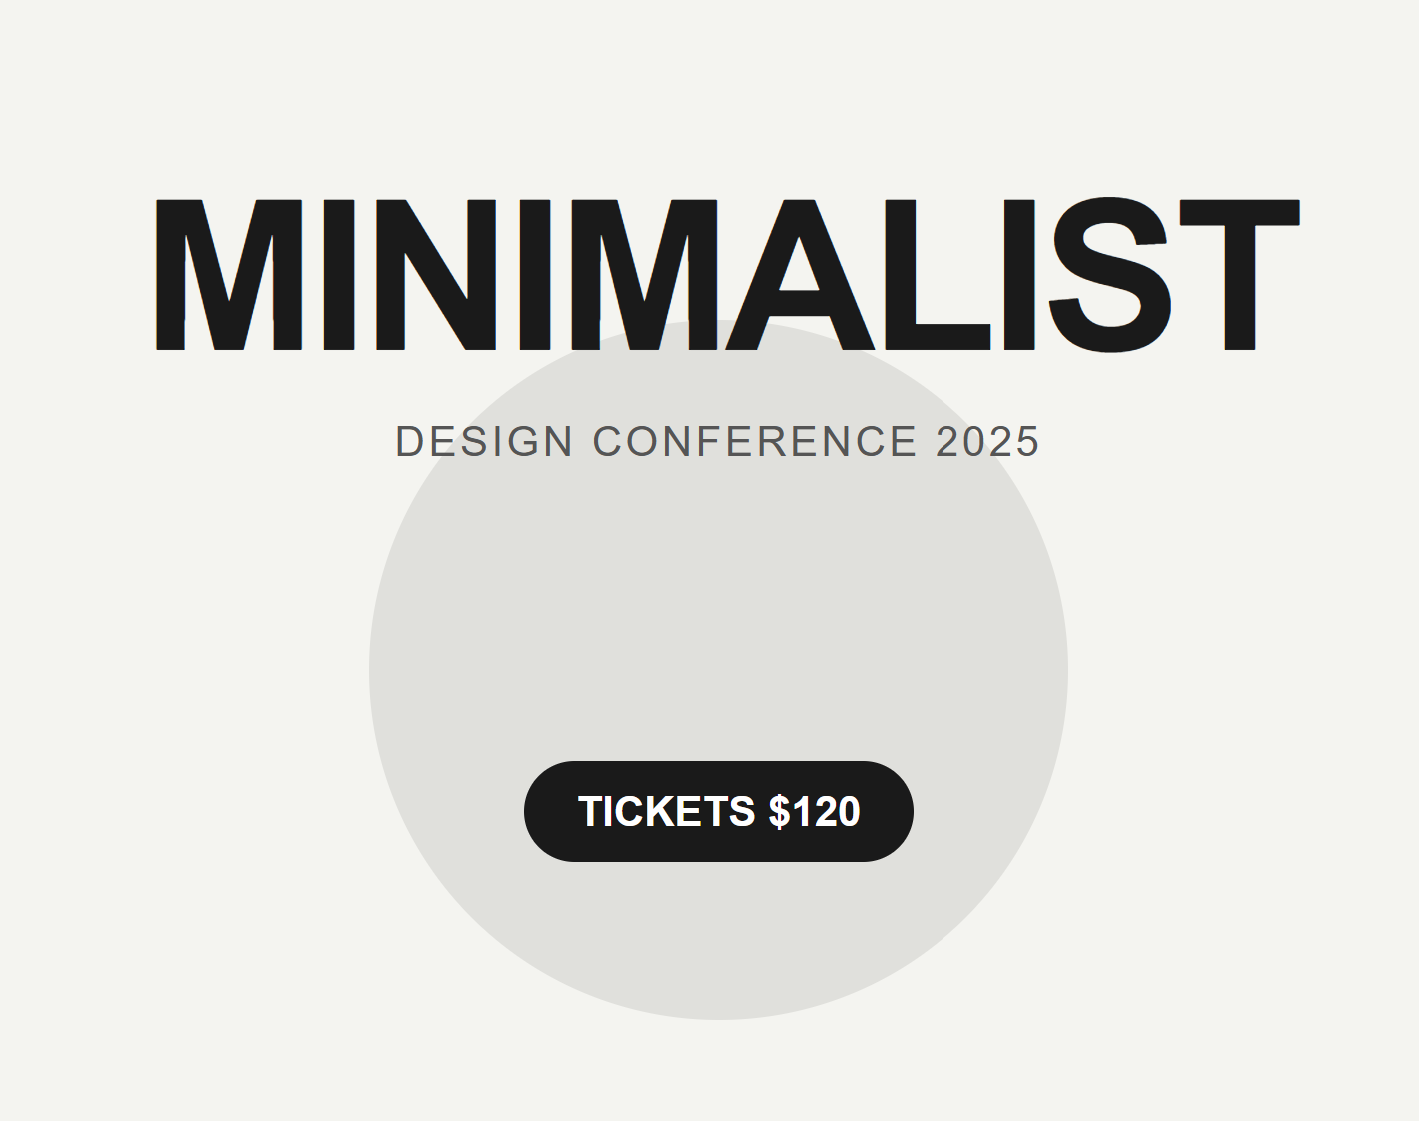
\includegraphics[width=0.8\linewidth]{images/ex_easy.png}
    \caption{Prompt: Change the color of the main title 'MINIMALIST' to bright blue hex code #3B82F6.}
    \label{fig:my_label}
\end{figure}

\begin{figure}[h]
    \centering
    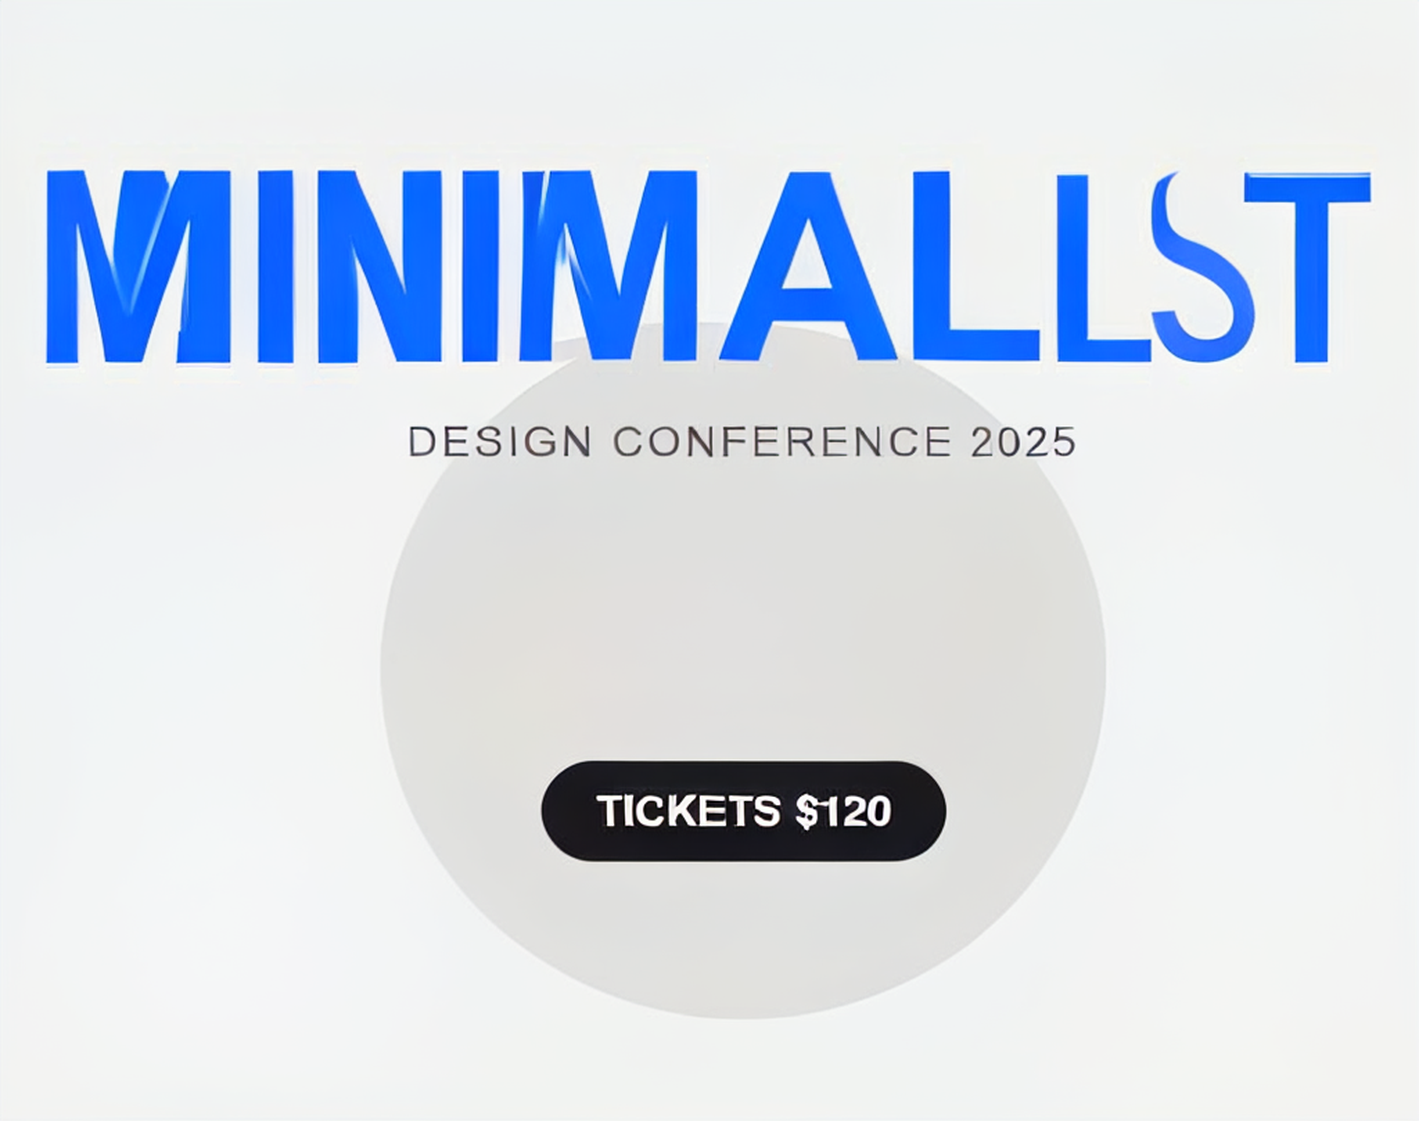
\includegraphics[width=0.8\linewidth]{images/varedit_output.png}
    \caption{VAREdit: Color is not exact, but quite close. The fonts and design "melts"}
    \label{fig:my_label}
\end{figure}

\begin{figure}[h]
    \centering
    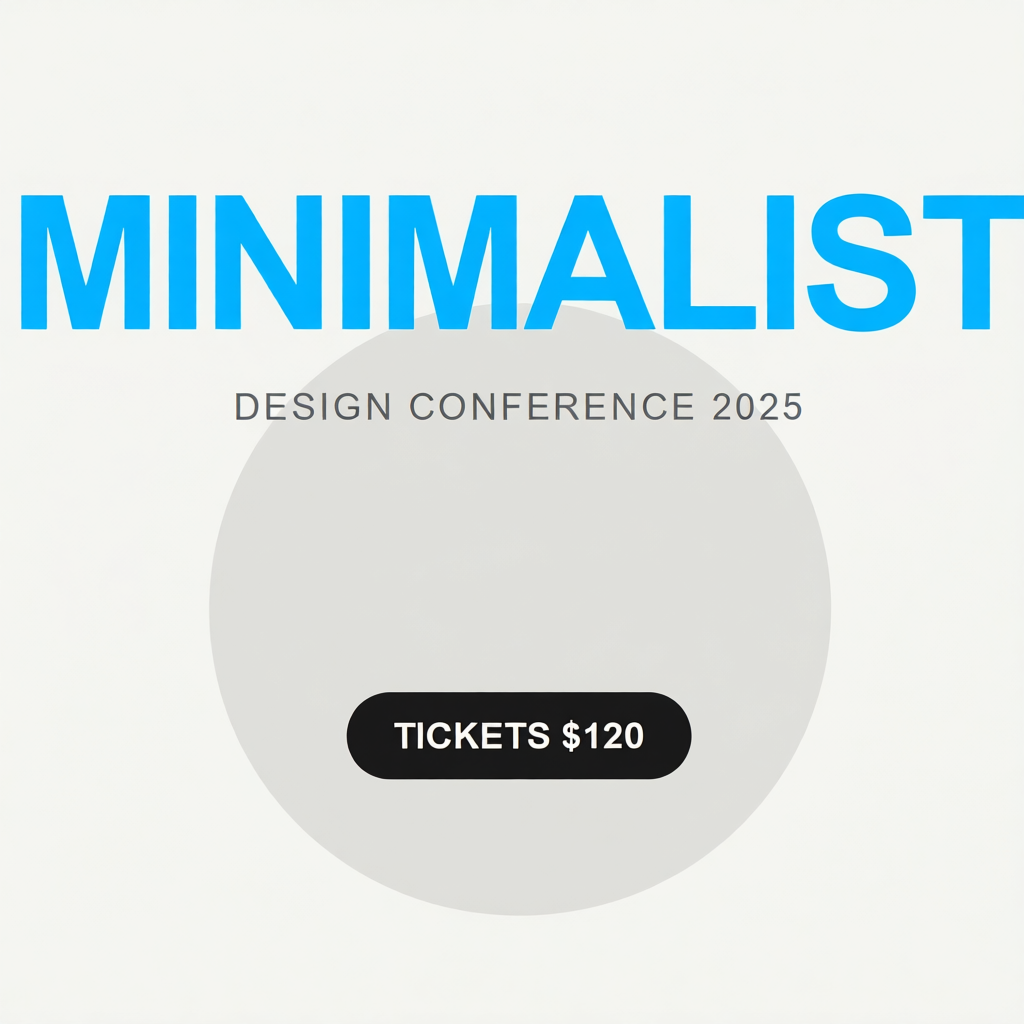
\includegraphics[width=0.8\linewidth]{images/qwen_output.png}
    \caption{QWen: Color is quite far away, otherwise result is very good. Makes me woner, does it use a bounding box and edits only a subsection of an image?}
    \label{fig:my_label}
\end{figure}

\begin{figure}[h]
    \centering
    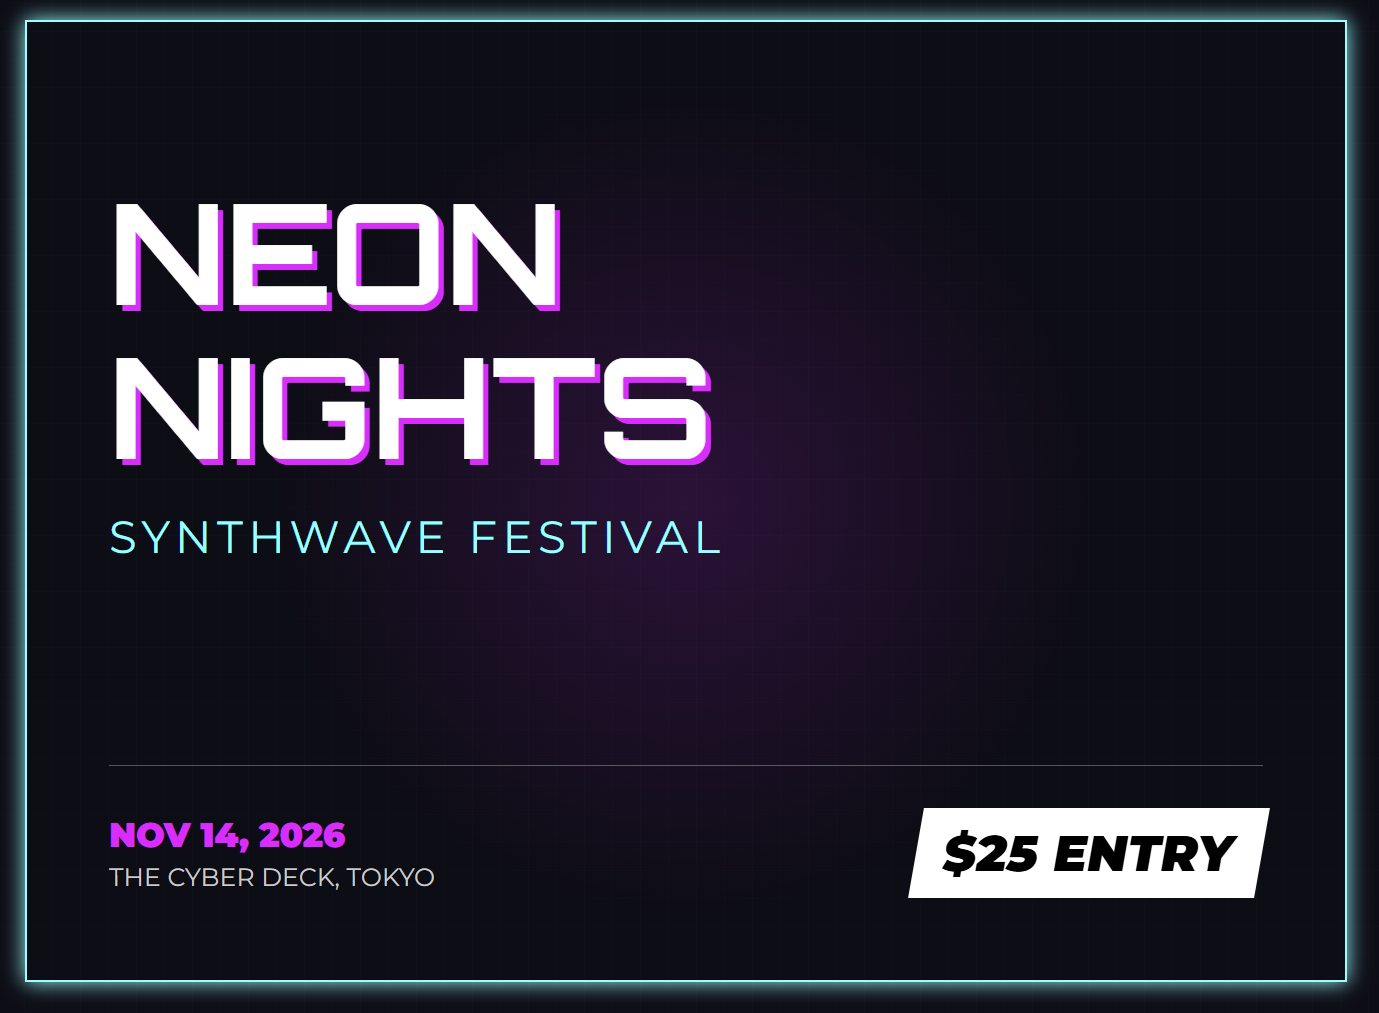
\includegraphics[width=0.8\linewidth]{images/ex_center.png}
    \caption{Center the title text horizontally within the poster}
    \label{fig:my_label}
\end{figure}

\begin{figure}[h]
    \centering
    
\includegraphics[width=0.8\linewidth]{images/varedit_output_center.png}
    \caption{Does not change much. But again details are melting}
    \label{fig:my_label}
\end{figure}

\begin{figure}[h]
    \centering
    
\includegraphics[width=0.8\linewidth]{images/qwen_output_center.png}
    \caption{Completely different design}
    \label{fig:my_label}
\end{figure}

%\input{file_name_of_chapter_x}
%\input{file_name_of_chapter_y}

% The thesis main content ends here.

\printbibliography

\begin{comment}
Important! Create the appendix chapters with command \textbackslash appchapter\{some
name\} instead of \textbackslash chapter\{some name\} for the automagic
page counting to work!
\end{comment}

\begin{comment}
\appchapter{Liitedokumentti}

Liitteen ohjelmakoodi \ref{alg:Tyyppiluokka-Monad} kuvaa matemaattisen
monadirakenteen pohjalta rakentuvan Haskellin tyyppiluokan. Tyyppiluokan
voi nähdä eräänlaisena abstraktina ohjelmointirajapintana (API\nomenclature[API]{API}{Application Programming Interface}),
joka muodostaa ohjelmoijalle abstraktin ohjelmointikielen käyttöliittymän
(UI\nomenclature[UI]{UI}{User Interface}).

\begin{algorithm}[tbh]
\begin{minted}{haskell}
class Monad m where
    ( >>= )         :: m a -> (a -> m b) -> m b
    return          :: a                 -> m a

    fail            :: String            -> m a
    (>>)            :: m a -> m b        -> m b
    m >> k          =  m >>= \_ -> k       -- default

instance Monad IO where  ...               -- omitted
\end{minted}

\caption{Tyyppiluokka 'Monad'.\label{alg:Tyyppiluokka-Monad}}
\end{algorithm}

\newpage{}

Ensimmäisen liitteen toinen sivu. Ohjelmalistaus \ref{alg:Monadin-kayttoa}
demonstroi vielä monadin käyttöä.

\begin{algorithm}[tbh]
\begin{minted}{haskell}
main =
return "Your name:" >>=
putStr >>=
\_ -> getLine >>=
\n -> putStrLn ("Hey " ++ n)
\end{minted}

\caption{Monadin käyttöä.\label{alg:Monadin-kayttoa}}
\end{algorithm}


\appchapter{Liitedokumentti 2}

Tässä esimerkki\pagebreak{}

toisesta kaksisivuisesta liitteestä.
\end{comment}
\end{document}
